\documentclass[lettersize, journal]{IEEEtran}

% ---------- PACKAGES ----------
\usepackage[utf8]{inputenc} % For UTF-8 encoding
\usepackage[T1]{fontenc}    % For accented characters
\usepackage{mathptmx}       % Times New Roman font
\usepackage{graphicx}       % For including images
\usepackage{float}          % For controlling float positions
\usepackage[ruled,vlined]{algorithm2e}
% \usepackage{caption}
% \usepackage{subcaption}
\usepackage{amsmath, amsfonts, amssymb} % Common math packages
\usepackage{hyperref}
\usepackage{enumitem}       % For customizable lists
\usepackage[caption=false,font=footnotesize,labelfont=sf,textfont=sf]{subfig}
% Use natbib for flexible in‑text citations (allows \citet and \citep) while keeping numeric IEEE style
% \usepackage{cite}
\usepackage[numbers,sort&compress]{natbib}
\usepackage{array}
\usepackage{balance}
\usepackage{tikz}           % For flowcharts or block diagrams
\usetikzlibrary{shapes,arrows.meta,positioning,calc,shadows,backgrounds,decorations.pathreplacing,fit,petri,arrows}
% \usetikzlibrary{shapes, arrows.meta, positioning, chains, fit, calc, shapes.geometric, shadows}
\usepackage{booktabs}       % For professional tables with \toprule, \midrule, etc.
\usepackage{multirow}       % For table cells spanning multiple rows
\usepackage{makecell}       % For better table cell formatting

% ---------- IEEEtran RECOMMENDATIONS ----------
\hyphenation{op-tical net-works semi-conduc-tor IEEE-Xplore}
\def\BibTeX{{\rm B\kern-.05em{\sc i\kern-.025em b}\kern-.08em
   T\kern-.1667em\lower.7ex\hbox{E}\kern-.125emX}}

% ---------- TITLE & AUTHOR ----------
\title{\textbf{MSAGAT-Net: An Efficient Multi-Scale Temporal Graph Attention Network for Spatiotemporal Epidemic Forecasting}}

% \author{
%     \IEEEauthorblockN{Author Names}
%     \IEEEauthorblockA{Institution\\
%     Email: author@institution.edu}
% }

% \markboth{IEEE Transactions on ...}{}

\author{
    \IEEEauthorblockN{
        Michael Ajao-olarinoye\IEEEauthorrefmark{1},~\IEEEmembership{Member,~IEEE,}
        Vasile Palade\IEEEauthorrefmark{1},~\IEEEmembership{Senior Member,~IEEE,}
        % Seyed Mosavi\IEEEauthorrefmark{1},~\IEEEmembership{Member,~IEEE,},
        Fei He\IEEEauthorrefmark{1}, 
        Zindoga Mukandavire\IEEEauthorrefmark{1},
        \textit{and}
        Petra Wark\IEEEauthorrefmark{2}
    }\\
    \IEEEauthorblockA{\IEEEauthorrefmark{1}Centre for Computational Science and Mathematical Modelling, Coventry University, Coventry, United Kingdom}\\
    \IEEEauthorblockA{\IEEEauthorrefmark{2}Research Institute for Health and Wellbeing, Coventry University, Coventry, United Kingdom}\\
    \IEEEauthorblockA{\IEEEauthorrefmark{3}Institute of Applied Research and Technology, Dubai International Academic City Dubai - UAE}
    % email for olarinoyem@coventry.ac.uk
    \IEEEauthorblockA{\{Email: olarinoyem@coventry.ac.uk\}}
}

\markboth{IEEE Journal of ......,~Vol.~XX, No.~YY, Month~Year}{}

% ---------- DOCUMENT BEGIN ----------
\begin{document}
\maketitle

% ---------- ABSTRACT ----------
\begin{abstract}
We present MSAGAT-Net, a novel Multi-Scale Temporal Graph Attention Network designed for accurate spatiotemporal epidemic forecasting across multiple geographical regions. Our approach addresses three critical challenges in epidemic prediction: (1) capturing complex spatial dependencies between regions with linear-time complexity, (2) modeling multi-scale temporal patterns in disease transmission, and (3) generating reliable multi-horizon forecasts. MSAGAT-Net introduces three key innovations: an Efficient Adaptive Graph Attention Module (EAGAM) that achieves O(N) complexity through linearized attention mechanisms and low-rank decomposition, a Dilated Multi-Scale Temporal Module (DMTM) that captures both short-term fluctuations and long-term trends, and a Progressive Prediction Module (PPM) for iterative multi-step forecasting. Through extensive experiments on diverse epidemic datasets spanning influenza and COVID-19 across multiple countries, MSAGAT-Net consistently outperforms state-of-the-art methods, achieving up to 23.7\% lower RMSE and 15.8\% higher correlation coefficients. Our ablation studies reveal disease-specific and horizon-dependent component importance patterns, providing insights into the varying spatiotemporal dynamics of different epidemics. The model's efficiency and interpretability make it particularly suitable for real-time public health surveillance and decision support systems.
\end{abstract}

% ---------- INDEX TERMS ----------
\begin{IEEEkeywords}
Deep Learning, Graph Neural Networks, Multi-head Attention, Time Series Analysis, Epidemic Forecasting, Adaptive Graph Learning, Multi-scale Feature Fusion, Spatiotemporal Prediction
\end{IEEEkeywords}

% ---------- SECTION I: INTRODUCTION ----------
\section{Introduction}

Spatio-temporal forecasting plays a critical role in addressing complex real-world problems, from urban traffic management and environmental monitoring to epidemic prediction and resource allocation. 
% Accurate forecasting in these domains requires models that can effectively capture both spatial dependencies between different geographical regions and temporal patterns within each region over time. 
The COVID-19 pandemic has underscored the importance of reliable epidemic forecasting models that can adapt to rapidly changing dynamics and provide actionable insights for timely public health decision-making and resource allocation \cite{ajao2023deep,da2021covid, giuliani2020modelling, verma2022temporal, ma2024reporting}. However, developing such models presents significant challenges due to the complex interplay between spatial dependencies, temporal patterns, and the inherent uncertainty in disease transmission.

A number of studies have explored forecasting in various domains, including traffic prediction \cite{li2017diffusion, zhang2021graph}, environmental monitoring \cite{wu2018deep, lai2018modeling}, and epidemic forecasting \cite{kimForecastingEpidemicSpread2025, zhiweidingBiologyInformedRecurrentNeural2023}. Using deep learning techniques, such as recurrent neural networks (RNN), convolutional neural networks (CNN), and graph neural networks (GNN), researchers have made significant strides in improving forecasting accuracy and efficiency, particularly in capturing complex patterns and relationships within the data.

However, existing approaches to spatiotemporal epidemic forecasting face several limitations. Traditional epidemiological models, such as compartmental SIR-based models, often struggle to capture the nuanced spatial relationships between regions and require extensive parameter tuning. Recent deep learning approaches have shown promise but suffer from computational inefficiencies when modeling spatial dependencies, particularly as the number of regions increases. Furthermore, most existing methods fail to adequately address the multi-scale nature of epidemic dynamics, where both short-term fluctuations and long-term trends play crucial roles in accurate forecasting.

In this paper we present MSAGAT-Net (Multi‑Scale Temporal Graph Attention Network), a compact and practical architecture that tackles the scalability and multi‑horizon challenges of epidemic forecasting by combining three complementary design choices. An Efficient Adaptive Graph Attention Module (EAGAM) replaces costly pairwise attention with a linearised, low‑rank formulation that learns interpretable inter‑region dependencies at O(N) cost. A Dilated Multi‑Scale Temporal Module (DMTM) captures dynamics at several temporal resolutions via dilated convolutions, allowing the model to represent both abrupt short‑term changes and slower seasonal trends. Finally, a Progressive Prediction Module (PPM) produces stable multi‑step forecasts by iteratively refining outputs using the most recent observations. Together these components form an efficient, interpretable framework suitable for real‑time epidemic surveillance and multi‑horizon prediction.

Our contributions are as follows:
\begin{enumerate}
\item We propose a computationally efficient graph attention mechanism that maintains modeling capacity while significantly reducing computational complexity through linearized attention and low-rank decomposition
\item We develop a multi-scale temporal processing framework that adaptively combines features from different temporal resolutions
\item We demonstrate through extensive experiments that MSAGAT-Net consistently outperforms state-of-the-art methods across diverse epidemic datasets
\item We provide comprehensive ablation studies revealing disease-specific and horizon-dependent patterns in component importance
\end{enumerate}


% ---------- SECTION II: LITERATURE REVIEW ----------
\section{Related Work}

Epidemiological forecasting has evolved considerably from traditional compartmental models such as SIR and SEIR, which, whilst providing valuable theoretical insights, often struggle to capture the complex spatial interactions and non-linear dynamics characteristic of real-world disease transmission \cite{lijingwangCausalGNNCausalBasedGraph2022}. The emergence of deep learning approaches has transformed this landscape, with graph neural networks proving particularly effective for modelling disease spread across interconnected regions by naturally representing locations as nodes and their interactions as edges.

The application of graph neural networks to epidemic forecasting addresses fundamental limitations of traditional approaches by learning complex spatiotemporal relationships directly from data. A comprehensive review by Liu et al. \cite{liuReviewGraphNeural2024a, wang_deepest_2024} categorises these methods into pure neural versus hybrid mechanistic-neural models, highlighting their growing significance in epidemiological research.

Deng et al. \cite{dengColaGNNCrosslocationAttention2020a} pioneered the use of dynamic cross-location attention mechanisms in their Cola-GNN framework for long-term influenza forecasting. Rather than relying on fixed geographic adjacency matrices, Cola-GNN learns adaptive attention weights between regions, effectively creating a dynamic graph that captures time-varying influences. This attention mechanism is coupled with dilated convolutional neural networks for temporal feature extraction, enabling the model to capture both short-term fluctuations and long-term patterns. The resulting framework not only improved multi-week ILI predictions but also provided interpretable insights into inter-regional influences.

Building upon these foundations, Xie et al. \cite{xie2022epignn} developed EpiGNN, which incorporates transmission risk encoding and a Region-Aware Graph Learner to model both local and global spatial effects. EpiGNN's architecture allows for the integration of external data sources, such as human mobility patterns, into the graph learning process. This approach demonstrated substantial improvements over previous state-of-the-art methods, achieving approximately 9.5\% reduction in RMSE across influenza and COVID-19 datasets.

Similarly, Gao et al. \cite{gao2021stan} proposed STAN (Spatio-Temporal Attention Network), which leverages attention-based graph convolution to capture dynamic geographical influences for COVID-19 forecasting. By incorporating patient electronic health record features and geography-based attention mechanisms, STAN successfully modelled spatial-temporal trends across all U.S. counties, significantly outperforming classical SIR/SEIR models with up to 87\% lower mean squared error. Notably, STAN incorporated physics-based regularisation terms derived from compartmental dynamics to improve long-range forecast stability.

The temporal dimension of epidemic forecasting presents unique challenges, as epidemic time series often exhibit complex seasonality, trends, and behavioural change effects. Current approaches to multi-step forecasting can be broadly categorised into direct methods, which predict multiple time steps simultaneously, and iterative methods, which generate forecasts sequentially.

Direct multi-horizon models, often implemented using sequence-to-sequence architectures with LSTM or CNN components, have demonstrated effectiveness in influenza forecasting but typically require substantial training data and may depend heavily on external covariates. Conversely, iterative strategies, whilst more data-efficient, suffer from error accumulation over extended forecasting horizons.

Deng et al. \cite{dengColaGNNCrosslocationAttention2020a} addressed long-term forecasting challenges by extracting multi-scale temporal features through dilated convolutions, finding that incorporating seasonal trends significantly improved forecast stability. Other researchers have explored hybrid approaches: Wu et al. \cite{wu2018deep} and Venna et al. \cite{venna2019novel} investigated direct long-term neural predictors for influenza, whilst Wang et al. \cite{wang2019defsi} developed DEFSI, which combines deep learning with compartmental models to enhance long-range forecasts.

The recognition of both short-term outbreaks and long-term epidemiological waves has led to the development of multi-module architectures that can simultaneously capture high-frequency fluctuations and low-frequency trends. These approaches often incorporate external data sources, including climate variables, demographic information, and digital surveillance indicators, to inform long-range predictions.

A particularly promising research direction involves the integration of epidemiological domain knowledge into deep learning frameworks to improve both interpretability and performance. Wang et al. \cite{lijingwangCausalGNNCausalBasedGraph2022} developed CausalGNN, which combines mechanistic ODE-based disease models with dynamic graph neural networks. In CausalGNN, an attention-based graph module captures cross-regional influences whilst a causal module, grounded in SIR-type ordinary differential equations, injects epidemiological context into node embeddings. This mutually-informed design yields more robust predictions with reduced parameter requirements.

Cao et al. \cite{cao2022mepognn} proposed MepoGNN, employing a multi-patch SEIR model within a metapopulation graph neural network framework. This approach merges region-level compartmental simulators with a Graph Attention Network that processes real-world mobility and case data, transforming static travel matrices into dynamic transmission adjacency matrices. When applied to COVID-19 spread in South Korea, MepoGNN demonstrated superior performance compared to pure simulation models, with learned transmission rates closely aligning with actual policy interventions.

Gao et al. \cite{gao2023evidence} took a physics-inspired approach with their HOIST model, drawing analogies between disease spread and Ising spin systems. By treating counties as nodes on a lattice and using Ising dynamics to regularise deep forecasting models, they encoded the principle that neighbouring regions' case counts should evolve in correlated patterns. Applied to 2,299 U.S. counties for four-week COVID-19 hospitalisation forecasting, HOIST achieved strong performance whilst providing policy-relevant insights, such as identifying rural vaccination strategies as particularly effective interventions.

Recent developments have focused on architectures that unify spatial and temporal modelling more deeply. Han et al. \cite{han2025dygraphformer} developed DyGraphFormer, integrating dynamic graph learning with Transformer architectures to capture evolving spatial-temporal dependencies. Unlike earlier models with fixed adjacency matrices, DyGraphFormer continuously updates its graph structure using recent historical data through gated recurrent units, allowing for adaptive representation of changing spatial dependencies.

Pu et al. \cite{pu2024dynamic} proposed the Dynamic Adaptive Spatio-Temporal Graph Network (DASTGN), which explicitly addresses mixed space-time relationships in epidemics through attention mechanisms that adaptively fuse spatial and temporal effects. DASTGN employs dual-scale attention: fine-grained modelling of time-specific and space-specific propagation influences, and coarse-grained capture of spatio-temporal neighbourhood blocks under varying intervention scenarios.

A critical practical consideration for large-scale epidemic forecasting is computational scalability. Traditional graph attention mechanisms among $N$ locations incur $O(N^2)$ computational complexity, which becomes prohibitive for fine-grained regional analysis. Recent advances in efficient attention, particularly linearised attention mechanisms that achieve $O(N)$ complexity through low-rank matrix decomposition called linformer by Wang et al. \cite{wang2020linformer}, offer promising solutions for real-time epidemic surveillance applications.


Despite these advances, several challenges remain in spatiotemporal epidemic forecasting. Current models often struggle to balance computational efficiency with modelling capacity, particularly when scaling to large numbers of regions. Many approaches fail to adequately capture multi-scale temporal dynamics, where both immediate fluctuations and long-term trends influence disease transmission. Additionally, most existing methods do not provide stable multi-horizon forecasting capabilities, which are essential for public health planning and resource allocation.

Our work addresses these gaps by developing MSAGAT-Net, which integrates efficient graph attention mechanisms, multi-scale temporal processing, and progressive prediction strategies. By combining insights from recent advances in linearised attention, adaptive graph learning, and multi-scale feature extraction, we aim to create a framework that maintains high accuracy whilst remaining computationally tractable for real-time deployment in public health surveillance systems.


% ---------- SECTION III: METHODOLOGY ----------
\section{Methodology}


\subsection{Problem Formulation}

Let us consider $N$ geographical regions (e.g., cities, counties, states, or NHS regions in England) as nodes in a graph. Historical epidemic data are represented as $\mathbf{X} = [\mathbf{x}_1, \mathbf{x}_2, \ldots, \mathbf{x}_T] \in \mathbb{R}^{N \times T}$, where $\mathbf{x}_t \in \mathbb{R}^N$ denotes the observed values in all $N$ regions at time step $t$. Each individual element $x_{i,t}$ represents the epidemic measure (e.g. ventilator bed occupancy or positive case count) for the region $i$ at time $t$.

For each specific region $i$, its temporal sequence is represented as $\mathbf{x}^i = [x_{i,1}, x_{i,2}, \ldots, x_{i,T}] \in \mathbb{R}^T$. This dual representation allows us to analyse both the spatial patterns (across regions at a specific time) and temporal patterns (within a region across time). 

Our primary objective is to predict future epidemic values for all regions on a specific time horizon $h$ steps ahead. Formally, given the historical data up to time $t$, we want to predict:

\begin{equation}
\mathbf{x}_{t+h} = [x_{1,t+h}, x_{2,t+h}, \ldots, x_{N,t+h}]^T
\end{equation}

For practical forecasting, we employ a sliding window approach with a fixed-length lookback period $w$. At any current time step $t$, we use the most recent observations $w$ $[\mathbf{x}_{t-w+1}, \mathbf{x}_{t-w+2}, \ldots, \mathbf{x}_t]$ to predict $\mathbf{x}_{t+h}$.

The spatial relationships between regions are encoded in a graph structure $\mathcal{G} = (\mathcal{V}, \mathcal{E}, \mathbf{A})$, where $\mathcal{V} = \{v_1, v_2, \ldots, v_N\}$ represents the set of regions, $\mathcal{E} \subseteq \mathcal{V} \times \mathcal{V}$ denotes the connections between regions and $\mathbf{A} \in \mathbb{R}^{N \times N}$ is the adjacency matrix. Each element $a_{ij}$ of $\mathbf{A}$ quantifies the strength of the relationship between regions $v_i$ and $v_j$. The adjacency matrix can be constructed based on various criteria, such as geographical proximity, transportation networks, or healthcare referral patterns. For example, in the context of epidemic forecasting, the adjacency matrix can reflect the mobility patterns of individuals between regions or the referral pathways of patients between healthcare facilities.

The forecasting task can be formalised as learning a function $f$ that maps recent historical data and graph structure to future predictions.

\begin{equation}
\mathbf{x}_{t+h} = f([\mathbf{x}_{t-w+1}, \mathbf{x}_{t-w+2}, \ldots, \mathbf{x}_t], \mathcal{G}; \boldsymbol{\Theta})
\end{equation}

where $\boldsymbol{\Theta}$ represents the learnable parameters of our forecasting model.

The challenge lies in designing this function $f$ to effectively capture both spatial dependencies between regions and temporal patterns within regions, whilst remaining computationally tractable and robust to the noisy and incomplete nature of epidemic data. Our approach, detailed in the following sections, addresses this challenge through a novel neural network architecture that combines graph attention mechanisms with multi-scale processing.

\begin{figure*}[htbp]
    \centering
    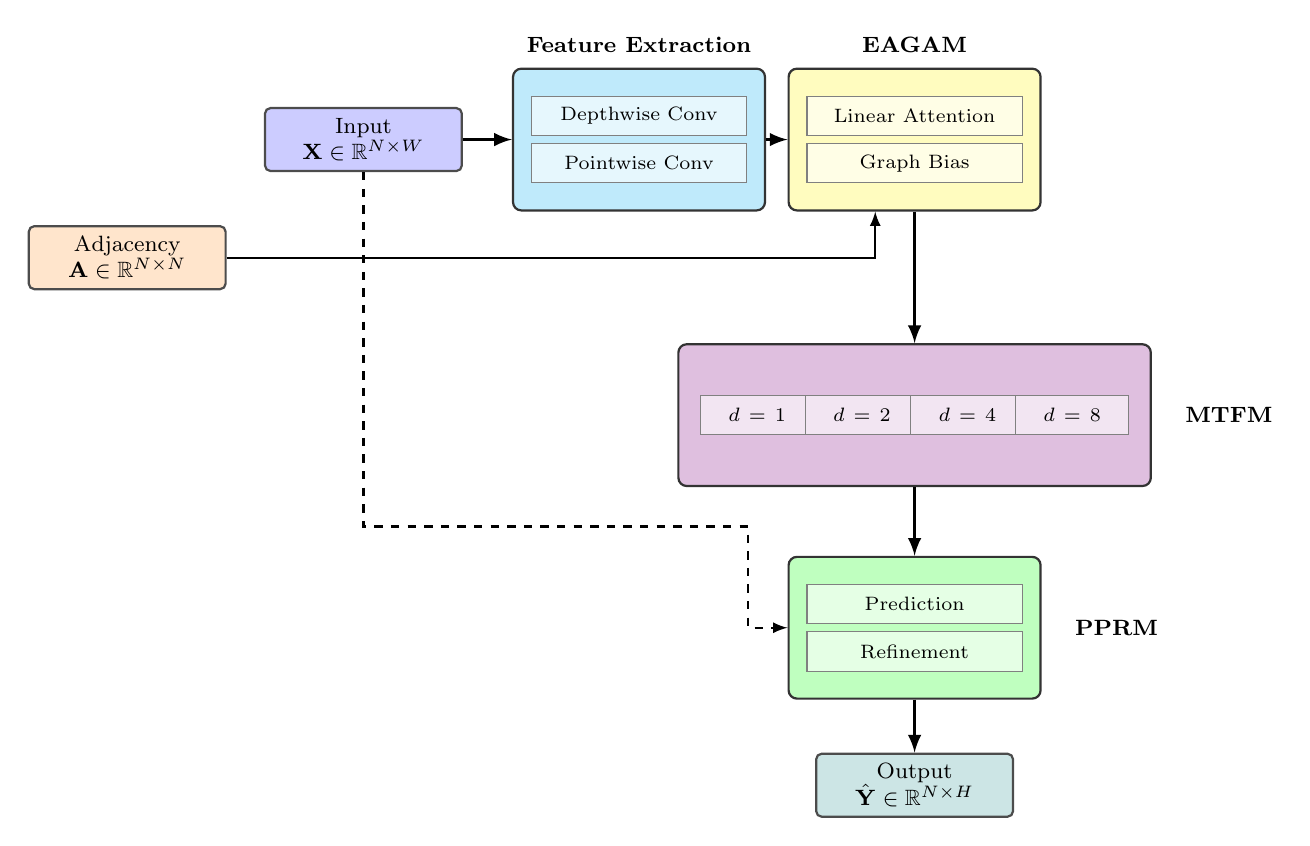
\begin{tikzpicture}[
        font=\footnotesize,
        >=latex,
        node distance = 1.5cm and 2.8cm,
        % Block styles
        module/.style={
            rectangle, 
            draw=black!80, 
            thick,
            rounded corners=3pt,
            minimum height=1.8cm, 
            minimum width=3.2cm,
            align=center,
            fill=#1!25
        },
        submodule/.style={
            rectangle, 
            draw=black!50, 
            minimum height=0.5cm, 
            text width=2.5cm,
            align=center,
            font=\scriptsize,
            fill=#1!10
        },
        data/.style={
            rectangle,
            draw=black!70,
            thick,
            rounded corners=2pt,
            minimum height=0.8cm,
            minimum width=2.5cm,
            align=center,
            fill=#1!20
        },
        arrow/.style={->, thick},
        bigarrow/.style={->, very thick},
        dashedarrow/.style={->, dashed, thick},
        label/.style={font=\footnotesize\bfseries}
    ]
    
    % Input
    \node[data=blue] (input) at (-5, 4) {Input\\$\mathbf{X} \in \mathbb{R}^{N \times W}$};
    \node[data=orange] (adj) at (-8, 2.5) {Adjacency\\$\mathbf{A} \in \mathbb{R}^{N \times N}$};
    
    % Feature Extraction
    \node[module=cyan] (feat) at (-1.5, 4) {};
    \node[label, above=2pt of feat] {Feature Extraction};
    \node[submodule=cyan] (dw) at ([yshift=0.3cm]feat.center) {Depthwise Conv};
    \node[submodule=cyan] (pw) at ([yshift=-0.3cm]feat.center) {Pointwise Conv};
    
    % AGAM
    \node[module=yellow] (eagam) at (2, 4) {};
    \node[label, above=2pt of eagam] {EAGAM};
    \node[submodule=yellow] (attn) at ([yshift=0.3cm]eagam.center) {Linear Attention};
    \node[submodule=yellow] (bias) at ([yshift=-0.3cm]eagam.center) {Graph Bias};

    % MTFM
    \node[module=violet, minimum width=6cm] (dmtm) at (2.0, 0.5) {}; % moved right from x=0.25 to x=2.25
    \node[label, above=2pt, right=0.3cm of dmtm] {MTFM};
    \node[submodule=violet, text width=1.2cm] (s1) at ([xshift=-2cm]dmtm.center) {$d=1$};
    \node[submodule=violet, text width=1.2cm] (s2) at ([xshift=-0.67cm]dmtm.center) {$d=2$};
    \node[submodule=violet, text width=1.2cm] (s3) at ([xshift=0.67cm]dmtm.center) {$d=4$};
    \node[submodule=violet, text width=1.2cm] (s4) at ([xshift=2cm]dmtm.center) {$d=8$};
    
    % PPRM
    \node[module=green] (ppm) at (2.0, -2.2) {};
    \node[label, above=2pt, right=0.3cm of ppm] {PPRM};
    \node[submodule=green] (pred) at ([yshift=0.3cm]ppm.center) {Prediction};
    \node[submodule=green] (refine) at ([yshift=-0.3cm]ppm.center) {Refinement};
    
    % Output
    \node[data=teal] (output) at (2.0, -4.2) {Output\\$\hat{\mathbf{Y}} \in \mathbb{R}^{N \times H}$};
    
    % Connections
    \draw[bigarrow] (input) -- (feat);
    \draw[bigarrow] (feat) -- (eagam);
    \draw[bigarrow] (eagam) -- (dmtm);
    \draw[bigarrow] (dmtm) -- (ppm);
    \draw[bigarrow] (ppm) -- (output);
    
    \draw[arrow] (adj) -| ([xshift=-0.5cm]eagam.south);
    \draw[dashedarrow] (input) |- ([yshift=-4.5cm]input.south) -| ([xshift=-0.5cm]ppm.west) -- (ppm);
    
    \end{tikzpicture}
    \caption{Overview of the MSAGAT-Net architecture. The model processes input through four main modules: Feature Extraction (depthwise separable convolutions), EAGAM (Efficient Adaptive Graph Attention Module with O(N) complexity), MTFM (Multi-scale Temporal Feature Module with dilation rates $d \in \{1,2,4,8\}$), and PPRM (Progressive Prediction Refinement Module). The dashed line represents the skip connection for refinement.}
    \label{fig:msagat_net_architecture}
\end{figure*}

\subsection{Feature Extraction}

The first component of the MSAGAT-Net architecture is the feature extraction module, which transforms the raw time-series data into meaningful feature representations whilst maintaining computational efficiency. Given the input time-series data $\mathbf{X} = [\mathbf{x}_{t-w+1}, \mathbf{x}_{t-w+2}, \ldots, \mathbf{x}_t] \in \mathbb{R}^{N \times w}$ for the $N$ regions over a lookback window of $w$ time steps, we need to extract features that capture relevant temporal patterns for each region. This is achieved through a combination of depthwise separable convolutions and low-rank projections, which allow for efficient feature extraction while reducing the risk of overfitting. The idea of using depthwise separable convolutions is inspired by the success of this approach in computer vision tasks, where it has been shown to significantly reduce the number of parameters and computational complexity while maintaining high performance \cite{chollet2017xception}. Our adaptation of this technique draws from the work of \cite{li2023multi} and \cite{yu2022traffic}, who have successfully applied depthwise separable convolutions to feature extraction rather than the standard convolutional approach. This allows us to efficiently capture the temporal dynamics of epidemic data without incurring the high computational costs associated with traditional convolutional architectures.

\subsubsection{Depthwise Separable Convolutions}

We employ the depthwise separable convolutions to extract temporal features efficiently. This approach significantly reduces the computational complexity and number of parameters whilst maintaining expressive power. The depthwise separable convolution consists of two stages:

For each region's time-series $\mathbf{x}^i \in \mathbb{R}^w$, the depthwise convolution applies a separate filter to each input channel (in this case, we treat the time-series as a single-channel input):

\begin{equation}
\mathbf{z}^i_{\text{depth}} = \text{Conv1D}_{\text{depth}}(\mathbf{x}^i; \boldsymbol{\Theta}_{\text{depth}})
\end{equation}

where $\mathbf{z}^i_{\text{depth}} \in \mathbb{R}^{w \times d_{\text{mid}}}$ represents the intermediate features after depthwise convolution, and $d_{\text{mid}}$ is the number of intermediate feature channels.

Following the depthwise convolution, a pointwise convolution (implemented as a 1×1 convolution) is applied to combine the features across channels:

\begin{equation}
\mathbf{z}^i_{\text{point}} = \text{Conv1D}_{\text{point}}(\mathbf{z}^i_{\text{depth}}; \boldsymbol{\Theta}_{\text{point}})
\end{equation}

where $\mathbf{z}^i_{\text{point}} \in \mathbb{R}^{w \times d_{\text{feat}}}$ represents the features after pointwise convolution, and $d_{\text{feat}}$ is the number of channels of output feature.

This decomposition significantly reduces the computational complexity and number of parameters compared to standard convolutions whilst maintaining similar expressive power. Specifically, for a standard convolution with kernel size $k$, input channels $c_{\text{in}}$, and output channels $c_{\text{out}}$, the parameter count is $k \times c_{\text{in}} \times c_{\text{out}}$. In contrast, the separable convolution in depth requires only $k \times c_{\text{in}} + c_{\text{in}} \times c_{\text{out}}$ parameters.

After each convolutional operation, we apply batch normalisation followed by ReLU activation to enhance training stability and introduce non-linearity:

\begin{equation}
\mathbf{z}^i_{\text{norm}} = \text{ReLU}(\text{BatchNorm}(\mathbf{z}^i_{\text{point}}))
\end{equation}

This normalisation step helps mitigate internal covariate shift during training, whilst the non-linear activation enables the model to capture complex temporal patterns in the epidemic data.

\subsubsection{Low-Rank Feature Projection}

After extracting features using depthwise separable convolutions, we applied a low-rank projection to further reduce dimensionality and capture the most salient features. This projection consists of two linear transformations with a bottleneck in between:

\begin{equation}
\mathbf{F}^i_{\text{low}} = \text{Linear}_{\text{low}}(\text{Flatten}(\mathbf{z}^i_{\text{norm}}))
\end{equation}

\begin{equation}
\mathbf{F}^i = \text{Linear}_{\text{high}}(\mathbf{F}^i_{\text{low}})
\end{equation}

where $\mathbf{F}^i_{\text{low}} \in \mathbb{R}^{d_{\text{bottle}}}$ is the bottleneck representation with dimension $d_{\text{bottle}}$, and $\mathbf{F}^i \in \mathbb{R}^{d_{\text{hidden}}}$ is the final representation of characteristics for region $i$ with dimension $d_{\text{hidden}}$.

The flattening operation converts the convolutional features $\mathbf{z}^i_{\text{norm}} \in \mathbb{R}^{w \times d_{\text{feat}}}$ into a vector of dimension $w \times d_{\text{feat}}$. This is then projected to the bottleneck dimension and subsequently to the hidden dimension.

After applying the low-rank projection to each region's convolutional features, we obtain a comprehensive feature matrix $\mathbf{F} \in \mathbb{R}^{N \times d_{\text{hidden}}}$, where each row $\mathbf{F}^i \in \mathbb{R}^{d_{\text{hidden}}}$ represents the temporal feature embedding for region $i$. This matrix encapsulates the essential temporal dynamics across all $N$ regions in a compact, information-dense representation suitable for subsequent spatial modelling.

The low-rank bottleneck projection ($w \times d_{\text{feat}} \to d_{\text{bottle}} \to d_{\text{hidden}}$) serves multiple critical functions within the architecture:

\begin{enumerate}
    \item By compressing information through a dimension bottleneck $d_{\text{bottle}} \ll w \times d_{\text{feat}}$, we reduce computational complexity from $\mathcal{O}(N \times w \times d_{\text{feat}} \times d_{\text{hidden}})$ to $\mathcal{O}(N \times (d_{\text{bottle}} \times d_{\text{hidden}} + w \times d_{\text{feat}} \times d_{\text{bottle}}))$, enabling efficient processing of large-scale spatio-temporal datasets.
    
    \item The bottleneck architecture creates an information bottleneck that forces the model to distill the most salient temporal patterns. This constrains the effective capacity of the network, preventing overfitting particularly when training data are limited relative to the high-dimensional input space.
    
    \item By forcing information through a lower-dimensional manifold, the projection encourages separation of relevant signals from noise, allowing subsequent layers to focus on truly predictive temporal patterns rather than spurious correlations.
    
    \item The shared projection parameters across all regions create a common latent space, facilitating meaningful comparison and interaction between region features in subsequent graph attention layers.
\end{enumerate}

To stabilise training and enhance feature quality, we apply layer normalisation followed by a non-linear activation:

\begin{equation}
\mathbf{F} = \text{ReLU}(\text{LayerNorm}(\mathbf{F}))
\end{equation}

The layer normalisation operates across the feature dimension, normalising each region's feature vector independently. This addresses internal covariate shift, enabling faster convergence during training whilst making the model robust to variations in feature scale across different regions. The ReLU activation introduces non-linearity essential for modelling complex temporal patterns whilst preserving sparse activation, a property particularly valuable for epidemic time-series that often exhibit punctuated patterns of activity against background stability.

This processed feature matrix $\mathbf{F}$ now encodes the essential temporal characteristics of each region's epidemic time-series in a form optimised for the subsequent Adaptive Graph Attention Module (AGAM), which will model dynamic spatial dependencies between regions based on these temporal feature representations. The feature extraction pipeline is illustrated in Figure~\ref{fig:feature_extraction}.

In our implementation, we set the default feature channel dimension $d_{\text{feat}}$ to 16, the bottleneck dimension $d_{\text{bottle}}$ to 8, and the hidden dimension $d_{\text{hidden}}$ to 32. These values were determined through ablation studies to balance model expressiveness with computational efficiency. For the convolutional operations, we use a kernel size of 3 with appropriate padding to maintain the temporal dimension. This combination of parameters enables our model to effectively capture temporal patterns whilst keeping the parameter count manageable, a crucial consideration for deployment in resource-constrained epidemic monitoring scenarios.

\begin{figure*}[htbp]
\centering
\resizebox{1.0\linewidth}{!}{%
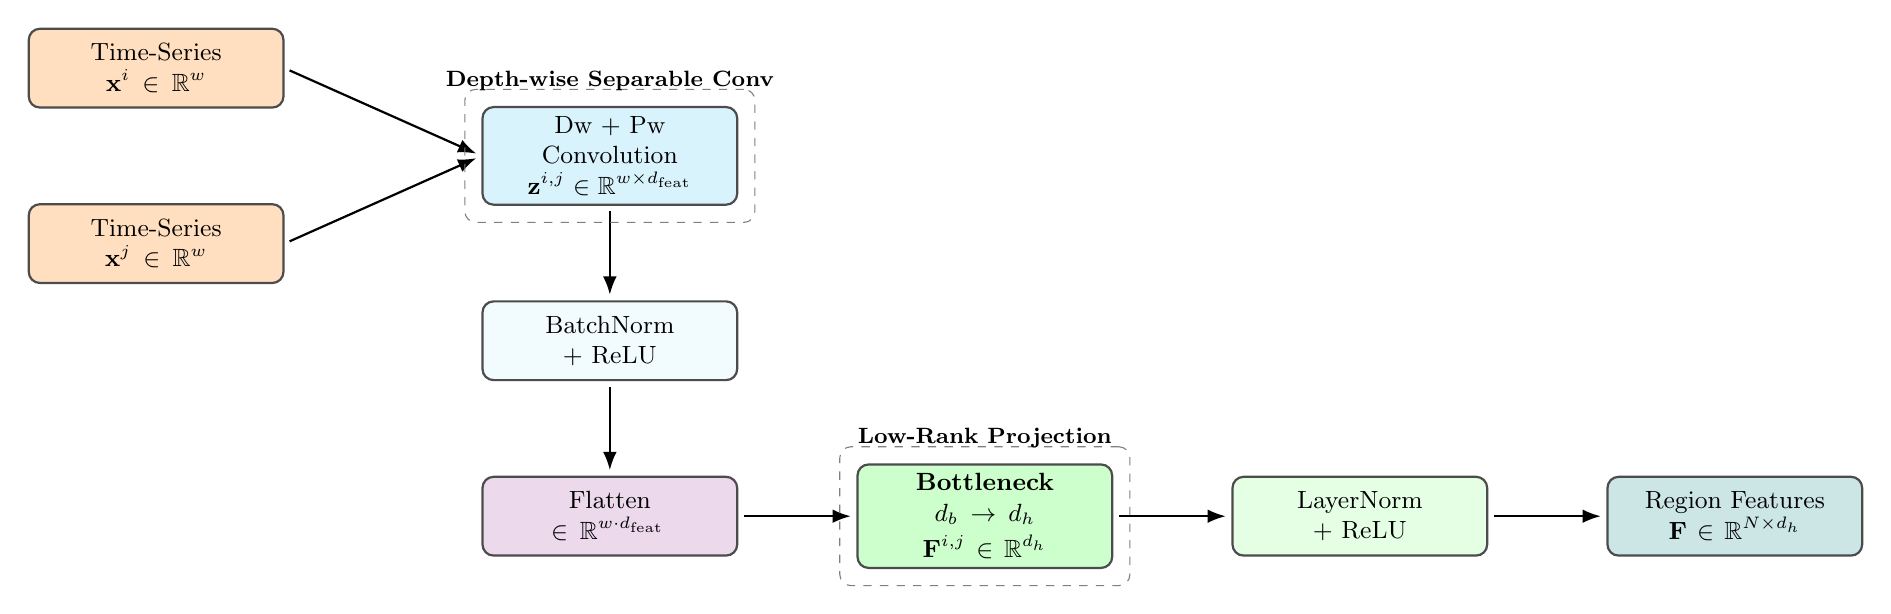
\begin{tikzpicture}[
    font=\small,
    >=Latex,
    block/.style={
        rectangle, draw=black!70, thick,
        rounded corners, align=center,
        minimum height=1cm,  % Increased height
        text width=3cm       % Increased width
    },
    arrow/.style={->, thick, shorten >=2pt, shorten <=2pt},
]
  %––– Inputs (split) –––––––––––––––––––––––––––––––––––––––
  \node (xi) [block, fill=orange!25] {Time‑Series\\$\mathbf{x}^i\!\in\!\mathbb{R}^{w}$};
  \node (xj) [block, fill=orange!25, below=1.2cm of xi] {Time‑Series\\$\mathbf{x}^j\!\in\!\mathbb{R}^{w}$};

  % Compute a point centred between xi and xj for tidy piping
  \path (xi.east) -- (xj.east) coordinate[midway] (midinput);

  %––– Pipeline nodes –––––––––––––––––––––––––––––––––––––––
  \node (sepconv) [block, fill=cyan!15,  right=2.5cm of midinput] {
      Dw + Pw\\Convolution\\
      $\mathbf{z}^{i,j}\!\in\!\mathbb{R}^{w\times d_{\text{feat}}}$};

  \node (bn)   [block, fill=cyan!5, below=1.2cm of sepconv] {BatchNorm\\+ ReLU};

  \node (flat) [block, fill=violet!15, below=1.2cm of bn] {Flatten\\$\!\in\!\mathbb{R}^{w\cdot d_{\text{feat}}}$};

  % Horizontal arrangement for the remaining nodes
  \node (proj) [block, fill=green!20, right=1.5cm of flat] {
      \textbf{Bottleneck}\\$d_b\!\to\! d_h$\\[2pt]
      $\mathbf{F}^{i,j}\!\in\!\mathbb{R}^{d_{h}}$};

  \node (ln) [block, fill=green!10, right=1.5cm of proj] {LayerNorm\\+ ReLU};

  \node (output) [block, fill=teal!20, right=1.5cm of ln] {Region Features\\$\mathbf{F}\!\in\!\mathbb{R}^{N\times d_{h}}$};

  %––– Arrows –––––––––––––––––––––––––––––––––––––––––––––––
  \draw[arrow] (xi.east) -- (sepconv.west);
  \draw[arrow] (xj.east) -- (sepconv.west);
  \draw[arrow] (sepconv.south) -- ++(0,-0.6) -- (bn.north);
  \draw[arrow] (bn.south) -- ++(0,-0.6) -- (flat.north);
  \draw[arrow] (flat.east) -- (proj.west);
  \draw[arrow] (proj.east) -- (ln.west);
  \draw[arrow] (ln.east) -- (output.west);

  %––– Grouping boxes –––––––––––––––––––––––––––––––––––––––
  \usetikzlibrary{fit}
  % \begin{scope}[on background layer] % Removed for IEEEtran compatibility
    \node[draw=black!50, dashed, rounded corners, inner sep=6pt,
          fit=(sepconv)] {};
    \node at (sepconv.north) [above=2pt, font=\footnotesize\bfseries] {Depth‑wise Separable Conv};

    \node[draw=black!50, dashed, rounded corners, inner sep=6pt,
          fit=(proj)] {};
    \node at (proj.north) [above=2pt, font=\footnotesize\bfseries] {Low‑Rank Projection};
  % \end{scope} % Removed for IEEEtran compatibility
\end{tikzpicture}%
}
\caption{Feature‑extraction pipeline. Independent regional time‑series $\mathbf{x}^i$ and $\mathbf{x}^j$ are processed in parallel by depth‑wise and point‑wise convolutions, normalised, flattened, passed through a bottleneck projection ($d_b\!\to\! d_h$), and normalised again to yield region‑level feature vectors $\mathbf F$.}
\label{fig:feature_extraction}
\end{figure*}

\subsection{Adaptive Graph Attention with Low-Rank Decomposition}

The second core component of our MSAGAT-Net architecture is the Adaptive Graph Attention Module (AGAM). Traditional approaches to spatial modelling often rely on fixed adjacency matrices based on geographical proximity or administrative boundaries, which do not capture the evolving nature of epidemic spread influenced by factors such as population mobility, healthcare referral patterns, and socioeconomic connections. Based on the principles of graph attention networks \cite{velickovic2017graph}, our AGAM adaptively learns the relationships between regions based on their feature representations, rather than being constrained by a predefined graph structure. This adaptive approach allows the model to discover and leverage spatial dependencies that may not be immediately apparent from geographical proximity alone, and to adjust these dependencies as the epidemic evolves.

A significant challenge in implementing graph attention mechanisms for large-scale epidemic or forecasting problems is computational complexity. Standard attention mechanisms in graph neural networks (GNNs) typically incur quadratic complexity with respect to the number of nodes, making them prohibitively expensive for large graphs. Additionally, these methods often suffer from over-smoothing when modelling long-range dependencies, where node representations become increasingly similar after multiple message-passing iterations.

Recent advances in efficient attention mechanisms have shown that low-rank decomposition techniques can substantially reduce computational complexity whilst maintaining expressive power. Several influential works have explored this direction. Researchers such as \cite{puny2020global} propose a low-rank global attention (LRGA), an adaptive module that replaces the total attention of the dot product in GNN with a decomposed low-rank form. \cite{kong2023low} present the Global Representation Key (GRK) attention layer, where the attention scores of each node are calculated using a shared projection of the features of its neighbours. A learnt adaptive low-rank matrix captures the most salient structural information, mitigating over-smoothing and improving performance on graphs. While \cite{yang2023self} embeds an adaptive low-rank decomposition step in each propagation layer within each ego network to concentrate message passing on the most prominent low-dimensional subspaces. This lets the model adaptively focus on the most informative subspace per node, improving robustness without labels. These studies collectively demonstrate that low‑rank factorisation offers an efficient, scalable and expressive alternative to full‑rank attention in graph architectures, and motivate the design of this module in our framework.

Motivated by these advances, AGAM employs a novel attention mechanism that combines low-rank decomposition with a learnable graph structure. Rather than computing the full attention matrix between all pairs of regions (which would incur $\mathcal{O}(N^2)$ complexity), we decompose the attention computation into more efficient operations. Specifically, we used a low-rank approximation of the attention matrix, which allows us to capture the most salient relationships between regions without incurring the full computational cost. This is achieved by projecting the feature representations into a lower-dimensional space before computing attention scores, effectively reducing the number of parameters and operations required.

This allows the model to adaptively learn the strength of connections between regions based on their feature representations rather than relying on a fixed adjacency matrix. The AGAM module consists of several key components: (1) low-rank feature projections, (2) multi-head attention computation, (3) enhanced attention stability, (4) learnable graph structure bias, and (5) attention regularisation. 

\subsubsection{Bottleneck Projection}

Given the feature matrix $\mathbf{F} \in \mathbb{R}^{N \times d_{\text{hidden}}}$ from the feature extraction module, where $N$ is the number of regions and $d_{\text{hidden}}$ is the hidden dimension, we first project these features into query, key, and value representations through an efficient bottleneck projection:

\begin{equation}
\mathbf{Q}_{\text{low}}, \mathbf{K}_{\text{low}}, \mathbf{V}_{\text{low}} = \text{Split}(\text{Linear}_{\text{low}}(\mathbf{F}), 3)
\end{equation}

where $\text{Linear}_{\text{low}}: \mathbb{R}^{d_{\text{hidden}}} \rightarrow \mathbb{R}^{3 \times d_{\text{bottle}}}$ projects the features into a lower-dimensional space and $\text{Split}$ divides the output into three separate tensors of dimension $\mathbb{R}^{N \times d_{\text{bottle}}}$.

These low-dimensional projections are then expanded back to the full hidden dimension:

\begin{equation}
\mathbf{Q}, \mathbf{K}, \mathbf{V} = \text{Split}(\text{Linear}_{\text{high}}([\mathbf{Q}_{\text{low}}; \mathbf{K}_{\text{low}}; \mathbf{V}_{\text{low}}]), 3)
\end{equation}

where $\text{Linear}_{\text{high}}: \mathbb{R}^{3 \times d_{\text{bottle}}} \rightarrow \mathbb{R}^{3 \times d_{\text{hidden}}}$ and each of $\mathbf{Q}, \mathbf{K}, \mathbf{V} \in \mathbb{R}^{N \times d_{\text{hidden}}}$.

This bottleneck projection significantly reduces the parameter count from $\mathcal{O}(3 \times d_{\text{hidden}}^2)$ to $\mathcal{O}(3 \times d_{\text{hidden}} \times d_{\text{bottle}})$, where $d_{\text{bottle}} \ll d_{\text{hidden}}$.

\subsubsection{Multi-Head Attention Mechanism}

To enhance the model's capacity to capture different types of inter-regional relationships, we implement a multi-head attention mechanism where the hidden representations are split into $h$ heads, each with dimension $d_{\text{head}} = d_{\text{hidden}} / h$:

\begin{equation}
\mathbf{Q}^{(i)}, \mathbf{K}^{(i)}, \mathbf{V}^{(i)} \in \mathbb{R}^{N \times d_{\text{head}}}, \quad i \in \{1, 2, \ldots, h\}
\end{equation}

For efficient computation, we reshape these tensors to explicitly represent the multiple heads:

\begin{equation}
\mathbf{Q}_h = \text{Reshape}(\mathbf{Q}, [N, h, d_{\text{head}}])
\end{equation}
\begin{equation}
\mathbf{K}_h = \text{Reshape}(\mathbf{K}, [N, h, d_{\text{head}}])
\end{equation}
\begin{equation}
\mathbf{V}_h = \text{Reshape}(\mathbf{V}, [N, h, d_{\text{head}}])
\end{equation}

We then transpose the first two dimensions to facilitate batch-wise processing across attention heads:

\begin{equation}
\mathbf{Q}_h, \mathbf{K}_h, \mathbf{V}_h = \text{Transpose}(\mathbf{Q}_h, 0, 1), \text{Transpose}(\mathbf{K}_h, 0, 1), \text{Transpose}(\mathbf{V}_h, 0, 1)
\end{equation}

resulting in tensors of shape $[h, N, d_{\text{head}}]$.

A key innovation in our approach is the specific attention computation mechanism employed within each head. Rather than relying on standard scaled dot-product attention with softmax, we employ an enhanced mechanism with better numerical stability and more nuanced relationship modelling.

First, we apply the Exponential Linear Unit (ELU) activation function followed by adding a constant value of 1 to both query and key representations:

\begin{equation}
\hat{\mathbf{Q}}_h = \text{ELU}(\mathbf{Q}_h) + 1
\end{equation}
\begin{equation}
\hat{\mathbf{K}}_h = \text{ELU}(\mathbf{K}_h) + 1
\end{equation}

This transformation ensures that all attention inputs are positive, improving gradient stability during training whilst allowing for more flexible attention patterns than the standard dot-product attention.

Next, we compute the key-value product for each attention head:

\begin{equation}
\mathbf{KV}_h = \hat{\mathbf{K}}_h^T \mathbf{V}_h
\end{equation}

where $\mathbf{KV}_h \in \mathbb{R}^{h \times d_{\text{head}} \times d_{\text{head}}}$. This operation captures the relationships between keys and values, allowing the model to learn how to weight the features of different regions based on their similarity.

To ensure stable normalisation, we calculate a normalisation factor based on the sum of keys:

\begin{equation}
\mathbf{z} = \frac{1}{\hat{\mathbf{K}}_h \cdot \mathbf{1} + \epsilon}
\end{equation}

where $\mathbf{1}$ is a vector of ones and $\epsilon$ is a small constant ($10^{-8}$ in our implementation) to prevent division by zero. This operation ensures stable normalisation across the attention heads, allowing for effective learning of inter-regional relationships. 

The final attention output for each head is computed as:

\begin{equation}
\mathbf{O}_h = \hat{\mathbf{Q}}_h \mathbf{KV}_h \mathbf{z}
\end{equation}

where $\mathbf{O}_h \in \mathbb{R}^{h \times N \times d_{\text{head}}}$ represents the attended features across all heads.

\subsubsection{Learnable Graph Structure}

An important feature of our AGAM is the incorporation of a learnable graph structure bias. Unlike traditional graph attention networks that rely solely on node features for computing attention, we include a learnable bias term that captures persistent structural relationships between regions that may not be evident from the node features alone.

This bias is implemented as a low-rank decomposition for parameter efficiency:

\begin{equation}
\mathbf{A}_{\text{bias}} = \mathbf{U} \mathbf{V}
\end{equation}

where $\mathbf{U} \in \mathbb{R}^{h \times N \times d_{\text{bias}}}$ and $\mathbf{V} \in \mathbb{R}^{h \times d_{\text{bias}} \times N}$ are learnable parameters and $d_{\text{bias}} \ll N$ is the bottleneck dimension of the bias term.

The bias is added to the computed attention scores before applying softmax:

\begin{equation}
\mathbf{A} = \text{softmax}\left(\frac{\hat{\mathbf{Q}}_h \hat{\mathbf{K}}_h^T}{\sqrt{d_{\text{head}}}} + \mathbf{A}_{\text{bias}}\right)
\end{equation}

This formulation allows the model to learn and encode persistent spatial dependencies between regions, such as geographical proximity or administrative hierarchies, whilst still adapting to data-driven patterns.

\subsubsection{Attention Regularisation}

To promote sparse and interpretable attention patterns, we apply L1 regularisation to the attention weights:

\begin{equation}
\mathcal{L}_{\text{attn}} = \lambda \|\mathbf{A}\|_1
\end{equation}

where $\lambda$ is the regularisation weight. This encourages the model to focus on the most relevant connections between regions, improving both interpretability and generalisation performance. The value of $\lambda$ (denoted as $\text{attention\_regularization\_weight}$ in our implementation) is treated as a hyperparameter and adjusted during model development.

After computing the attended values for each head, we combine them and project back to the original feature dimension:

\begin{equation}
\mathbf{O} = \text{Reshape}(\text{Transpose}(\mathbf{O}_h, 0, 1), [N, d_{\text{hidden}}])
\end{equation}

Similarly to the input projection, we employ a low-rank output projection for efficiency:

\begin{equation}
\mathbf{O}_{\text{low}} = \text{Linear}_{\text{out\_low}}(\mathbf{O})
\end{equation}

\begin{equation}
\mathbf{O}_{\text{final}} = \text{Linear}_{\text{out\_high}}(\mathbf{O}_{\text{low}})
\end{equation}

where $\mathbf{O}_{\text{low}} \in \mathbb{R}^{N \times d_{\text{bottle}}}$ and $\mathbf{O}_{\text{final}} \in \mathbb{R}^{N \times d_{\text{hidden}}}$.

The output of the AGAM, $\mathbf{O}_{\text{final}}$, represents the features of the region after incorporating spatial dependencies. This output, along with the attention regularisation loss $\mathcal{L}_{\text{attn}}$, is passed to the subsequent multi-scale Fusion Module for further processing.

% \subsubsection{Implementation Details}

In our implementation, we set the number of attention heads $h=4$ and the bottleneck dimension $d_{\text{bottle}}=8$ as default values. These were determined through ablation studies to provide an optimal balance between model expressiveness and computational efficiency. The weight of attention regularisation $\lambda$ is set to $10^{-5}$, which we found effectively promotes sparse attention patterns without overly constraining the model. The \autoref{fig:agam_module} image below represents the flow of data in the 

% The AGAM module introduces several key advantages for epidemic forecasting:

% \begin{enumerate}
%     \item \textbf{Adaptive spatial modelling}: By learning attention weights dynamically, the model can adapt to changing spatial dependencies over time, crucial for capturing evolving epidemic spread patterns.
    
%     \item \textbf{Computational efficiency}: The low-rank projections and decompositions significantly reduce the parameter count and computational complexity, enabling the model to scale to large numbers of regions.
    
%     \item \textbf{Interpretability}: The learnt attention patterns can provide valuable insights into region-to-region influence, potentially helping epidemiologists identify key transmission pathways.
    
%     \item \textbf{Integration of prior knowledge}: The learnable graph structure bias allows the model to incorporate domain knowledge about regional connections whilst still adapting to data-driven patterns.
% \end{enumerate}

% Through these innovations, the AGAM effectively captures the complex spatial dependencies inherent in epidemic data, providing a solid foundation for the subsequent temporal modelling steps in our architecture.


\begin{figure*}[htbp]
\centering
%–— 1. We still fix the width to \linewidth; the height now shrinks naturally –—
\resizebox{\linewidth}{!}{%
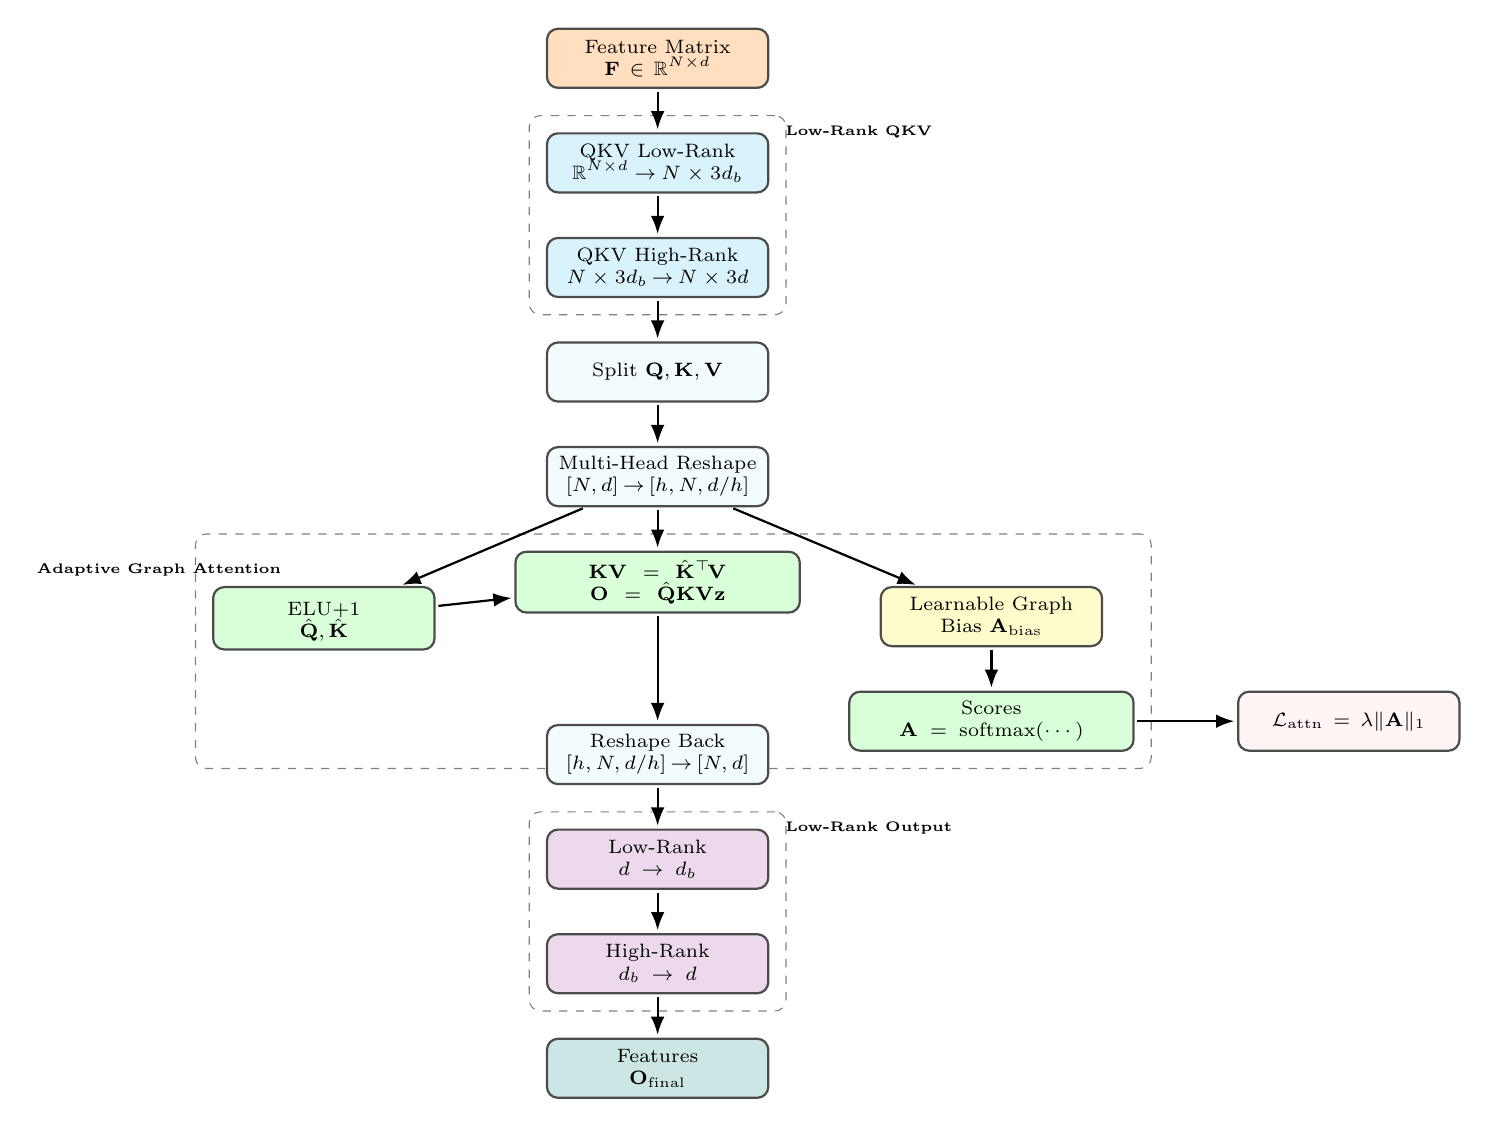
\begin{tikzpicture}[
    %–––– GLOBAL STYLE TWEAKS ––––
    font=\scriptsize,                                % smaller text
    >=Latex,
    node distance = 0.55cm and 1.6cm,                % default vert / horiz gap
    block/.style = {rectangle, draw=black!70, thick,
                    rounded corners, align=center,
                    minimum height=0.75cm,           % lower boxes
                    text width=2.6cm,                % narrower boxes
                    inner sep=3pt},                  % tighter padding
    wideblock/.style = {block, text width=3.4cm},    % a bit wider
    arrow/.style = {->, thick, shorten >=1pt, shorten <=1pt},
]
%–––– MAIN FLOW ––––
\node (input)      [block, fill=orange!25] {Feature Matrix\\$\mathbf{F}\!\in\!\mathbb{R}^{N\times d}$};

\node (qkv_low)    [block,  fill=cyan!15,  below=of input]          {QKV Low‑Rank\\$\mathbb{R}^{N\times d}\!\to\! N\times3d_b$};

\node (qkv_high)   [block,  fill=cyan!15,  below=of qkv_low]        {QKV High‑Rank\\$N\times3d_b\!\to\! N\times3d$};

\node (split)      [block,  fill=cyan!5,   below=of qkv_high]       {Split $\mathbf Q,\mathbf K,\mathbf V$};

\node (reshape)    [block,  fill=cyan!5,   below=of split]          {Multi‑Head Reshape\\$[N,d]\!\to\![h,N,d/h]$};

%–––– PARALLEL BRANCH (three nodes at same depth) ––––
\node (qk_proc)    [block,  fill=green!15, below left=1.0cm and 1.4cm of reshape] {\rule{0pt}{0.9em}ELU$+1$\\$\hat{\mathbf Q},\hat{\mathbf K}$};

\node (graph_bias) [block,  fill=yellow!20, below right=1.0cm and 1.4cm of reshape] {Learnable Graph\\Bias $\mathbf A_{\text{bias}}$};

\node (attn_comp)  [wideblock, fill=green!15, below=of reshape]     {$\mathbf{KV}=\hat{\mathbf K}^\top\!\mathbf V$\\
                                                                     $\mathbf O=\hat{\mathbf Q}\mathbf{KV}\mathbf z$};

%–––– ATTENTION SCORE / REG ––––
\node (attn_scores)[wideblock, fill=green!15, below=of graph_bias]  {Scores\\$\mathbf A=\text{softmax}( \cdots )$};

\node (attn_reg)   [block,      fill=pink!15,  right=1.3cm of attn_scores] {$\mathcal L_{\text{attn}}=\lambda\|\mathbf A\|_1$};

%–––– OUTPUT PATH ––––
\node (reshape_out) [block, fill=cyan!5,   below=1.4cm of attn_comp] {Reshape Back\\$[h,N,d/h]\!\to\![N,d]$};

\node (out_low)     [block, fill=violet!15, below=of reshape_out]   {Low‑Rank\\$d\!\to\! d_b$};

\node (out_high)    [block, fill=violet!15, below=of out_low]       {High‑Rank\\$d_b\!\to\! d$};

\node (output)      [block, fill=teal!20,   below=of out_high]      {Features\\$\mathbf O_{\text{final}}$};

%–––– ARROWS ––––
\foreach \a/\b in {
  input/qkv_low, qkv_low/qkv_high, qkv_high/split, split/reshape,
  reshape/qk_proc,  reshape/attn_comp, reshape/graph_bias,
  qk_proc/attn_comp, graph_bias/attn_scores,
  attn_scores/attn_reg, attn_comp/reshape_out,
  reshape_out/out_low, out_low/out_high, out_high/output}
  \draw[arrow] (\a) -- (\b);

%–––– GROUP BOXES (dashed) ––––
\usetikzlibrary{fit}
\begin{scope}[on background layer]
  \node [draw=black!50, dashed, rounded corners, inner sep=6pt,
         fit=(qkv_low)(qkv_high)] {};
  \node at (qkv_low.north) [above=1pt, right=0pt and 1.5cm, font=\tiny\bfseries] {Low‑Rank QKV};

  \node [draw=black!50, dashed, rounded corners, inner sep=6pt,
         fit=(qk_proc)(attn_comp)(graph_bias)(attn_scores)] {};
  \node at (qk_proc.north west) [above left=0pt and -1.0cm, font=\tiny\bfseries] {Adaptive Graph Attention};

  \node [draw=black!50, dashed, rounded corners, inner sep=6pt,
         fit=(out_low)(out_high)] {};
  \node at (out_low.north) [above=1pt, right=0pt and 1.5cm, font=\tiny\bfseries] {Low‑Rank Output};
\end{scope}
\end{tikzpicture}}%
\caption{Flow of data and structure in the AGAM module.}
\label{fig:agam_module}
\end{figure*}

Figure \ref{fig:agam_module} illustrates the flow of data through the AGAM module. The input feature matrix $\mathbf{F}$ is processed through low-rank projections to obtain query, key, and value representations. These representations are then reshaped for multi-head attention computation, where the adaptive graph attention mechanism is applied. The learnable graph structure bias is incorporated into the attention scores, and L1 regularisation is applied to promote sparse attention patterns. Finally, the output features are obtained through high-rank projections, ready for further processing in the multi-scale Fusion Module.

\subsection{Multi-scale Fusion Module}

The third major component of our MSAGAT-Net architecture is the multi-scale Fusion Module (MTFM), which addresses a fundamental challenge in epidemic forecasting: capturing temporal patterns that operate at different time scales simultaneously. 
Epidemics often show intricate temporal dynamics with various scales, including short-term changes (such as weekend effects), medium-term patterns (like incubation periods), and long-term trends (e.g., seasonal variations). Accurate forecasting depends heavily on effectively modelling these multi-scale dynamics.

Deng et al. \cite{dengColaGNNCrosslocationAttention2020a} introduce the idea of multi-scale dilated convolutional with the same filter and stride sides but different dilation rate, which Xie et al. \cite{xie2022epignn} improved on by making use of the multi-scale convolution to capture features. Building on this, the MTFM employs parallel dilated convolutional layers to efficiently capture temporal dependencies across multiple scales using the output from the AGAM. This approach enables the model to maintain an awareness of both immediate and distant temporal relationships whilst controlling parameter count and computational complexity.


\subsubsection{Dilated Convolutions for Multi-scale Processing}

The core of our MTFM is a set of parallel convolutional branches operating at different dilation rates. For a given input feature tensor $\mathbf{G} \in \mathbb{R}^{B \times N \times d_{\text{hidden}}}$ (where $B$ is the batch size, $N$ is the number of regions, and $d_{\text{hidden}}$ is the hidden dimension), we first transpose the tensor to prepare for 1D convolutions along the temporal dimension:

\begin{equation}
\mathbf{G}_{\text{conv}} = \text{Transpose}(\mathbf{G}, 1, 2)
\end{equation}

resulting in a tensor of shape $[B, d_{\text{hidden}}, N]$. We then process this tensor through $S$ parallel branches, each consisting of a dilated convolutional layer with a specific dilation rate, followed by batch normalisation, ReLU activation and dropout:

\begin{equation}
\mathbf{H}^{(i)} = \text{Dropout}(\text{ReLU}(\text{BatchNorm}(\text{Conv1D}(\mathbf{G}_{\text{conv}}; k, d^{(i)}))))
\end{equation}

where $i \in \{1, 2, \ldots, S\}$ indexes the scale, $k$ is the kernel size (set to 3 by default), and $d^{(i)} = 2^{i-1}$ is the dilation rate for the scale $i$. Each branch produces an output tensor $\mathbf{H}^{(i)} \in \mathbb{R}^{B \times d_{\text{hidden}} \times N}$.

The increasing dilation rates create an exponentially expanding receptive field across the branches:
\begin{itemize}
    \item Scale 1 ($d^{(1)} = 1$): Captures immediate temporal dependencies with a receptive field of $k$ time steps
    \item Scale 2 ($d^{(2)} = 2$): Captures medium-range dependencies with a receptive field of $k + (k-1)$ time steps
    \item Scale 3 ($d^{(3)} = 4$): Captures longer-range dependencies with a receptive field of $k + 3(k-1)$ time steps
    \item And so on for higher scales
\end{itemize}

This multi-scale approach allows the model to efficiently capture a wide range of temporal dependencies without requiring deep sequential processing, which is particularly advantageous for epidemic time-series that often exhibit both rapid changes and gradual trends.

\subsubsection{Adaptive Scale Fusion}

Rather than simply concatenating or averaging the outputs from different scales, we implement an adaptive fusion mechanism that allows the model to learn the relative importance of each temporal scale. This is achieved through learnable fusion weights:

\begin{equation}
\boldsymbol{\alpha} = \text{softmax}(\mathbf{w})
\end{equation}

where $\mathbf{w} \in \mathbb{R}^S$ is a learnable parameter vector and $\boldsymbol{\alpha} \in \mathbb{R}^S$ represents the normalised importance weights for each scale.

The multi-scale features are then fused using these weights:

\begin{equation}
\mathbf{H}_{\text{fused}} = \sum_{i=1}^{S} \alpha_i \mathbf{H}^{(i)}
\end{equation}

where $\mathbf{H}_{\text{fused}} \in \mathbb{R}^{B \times d_{\text{hidden}} \times N}$ is the scale-fused feature representation.

This adaptive fusion mechanism offers several advantages. It allows the model to automatically adjust the importance of different temporal scales based on the data, can adapt to different regions that might exhibit varying temporal characteristics, and provides interpretable insights into which temporal scales are most relevant for forecasting.

\begin{figure*}[htbp]
\centering
\includegraphics[width=0.7\textwidth]{figs/mtfm_diagram.pdf}
\caption{Flow of data in the MTFM architecture.}
\label{fig:mtfm_module}
\end{figure*}

\subsubsection{Bottleneck Projection and Residual Connection}

To enhance training stability and allow for more effective feature transformation, we apply a low-rank bottleneck projection to the fused features:

\begin{equation}
\mathbf{H}_{\text{low}} = \text{Linear}_{\text{fusion\_low}}(\text{Transpose}(\mathbf{H}_{\text{fused}}, 1, 2))
\end{equation}

\begin{equation}
\mathbf{H}_{\text{proj}} = \text{Linear}_{\text{fusion\_high}}(\mathbf{H}_{\text{low}})
\end{equation}

where $\mathbf{H}_{\text{low}} \in \mathbb{R}^{B \times N \times d_{\text{bottle}}}$ is the bottleneck representation with dimension $d_{\text{bottle}} \ll d_{\text{hidden}}$, and $\mathbf{H}_{\text{proj}} \in \mathbb{R}^{B \times N \times d_{\text{hidden}}}$ is the projected representation.

We then apply layer normalisation and a residual connection to facilitate gradient flow during training:

\begin{equation}
\mathbf{H}_{\text{final}} = \text{LayerNorm}(\text{Transpose}(\mathbf{H}_{\text{fused}}, 1, 2) + \mathbf{H}_{\text{proj}})
\end{equation}

where $\mathbf{H}_{\text{final}} \in \mathbb{R}^{B \times N \times d_{\text{hidden}}}$ is the final output of the MTFM.

In our implementation, the number of temporal scales $S$ is set to 4 by default, with dilation rates of $\{1, 2, 4, 8\}$. This configuration allows the model to capture dependencies ranging from immediate neighbours to relationships spanning up to 17 time steps ($3 + 7 \times 2 = 17$ with kernel size 3), which is sufficient for most epidemic forecasting applications given our sliding-window approach.

The kernel size $k$ is set to 3, providing a good balance between capturing local patterns and maintaining computational efficiency. The hidden dimension $d_{\text{hidden}}$ is maintained throughout the module to preserve the information capacity, while the bottleneck dimension $d_{\text{bottle}}$ is set to $d_{\text{hidden}} / 4$ to reduce the parameters in the projection layers.

To avoid overfitting, we apply dropout with probability 0.355 after each convolutional layer and ReLU activation. This relatively high dropout rate was determined by cross-validation to be effective for epidemic data, which can be noisy and prone to overfitting. The \autoref{fig:mtfm_module} presents a detailed representation of the architecture of this module. 


\subsection{Progressive Multi-step Prediction Refinement}

The final component of our MSAGAT-Net architecture is the Progressive Refinement Multi-step Prediction Module (PPRM), which addresses the critical challenge of generating accurate forecasts across multiple future time steps. Whilst the preceding modules excel at extracting spatio-temporal features, converting these features into reliable predictions, particularly for longer horizons, requires additional consideration of how prediction errors can compound over time and how recent observations might inform future trajectory adjustments.

The PPRM addresses the critical issue of error accumulation inherent in multi-horizon epidemiological forecasting. Through an extensive analysis of multistep forecasting failures, it became evident that prediction errors compound exponentially with increasing prediction horizons \citep{BENTAIEB20127067, chandra2021evaluation}. This module incorporates concepts from residual error correction, ensemble learning, and adaptive gating mechanisms common in recurrent neural network architectures \citep{hochreiter1997long}.

The PPRM takes the rich spatio-temporal representations from previous modules and transforms them into horizon-specific predictions, incorporating an adaptive refinement mechanism that balances model-based forecasts with data-driven trends. This design is motivated by epidemiological observations that disease progression often follows certain patterns based on a recent trajectory, even as it responds to various complex factors captured by our neural network components.

\subsubsection{Low-Rank Prediction Projection}

Given the spatio-temporal feature tensor $\mathbf{H}_{\text{final}} \in \mathbb{R}^{B \times N \times d_{\text{hidden}}}$ from the multi-scale Fusion Module, where $B$ is the batch size, $N$ is the number of regions, and $d_{\text{hidden}}$ is the hidden dimension, we first apply a bottleneck projection to distil the most forecast-relevant information:

\begin{equation}
\mathbf{P}_{\text{low}} = \text{Linear}_{\text{pred\_low}}(\mathbf{H}_{\text{final}})
\end{equation}

where $\mathbf{P}_{\text{low}} \in \mathbb{R}^{B \times N \times d_{\text{bottle}}}$ is the bottleneck representation with dimension $d_{\text{bottle}} \ll d_{\text{hidden}}$.

This bottleneck projection serves multiple purposes:
\begin{enumerate}
    \item It reduces the parameter count in the subsequent prediction layers
    \item It forces the model to identify the most salient features for forecasting
    \item It acts as an implicit regulariser, helping to prevent overfitting
\end{enumerate}

We then apply layer normalisation, ReLU activation, and dropout to the bottleneck representation:

\begin{equation}
\mathbf{P}_{\text{mid}} = \text{Dropout}(\text{ReLU}(\text{LayerNorm}(\mathbf{P}_{\text{low}})))
\end{equation}

This intermediate processing enhances training stability and introduces non-linearity necessary for modelling complex forecast patterns.

\subsubsection{Horizon-Specific Prediction}

From the processed bottleneck representation, we generate initial predictions for all forecast horizons using a linear projection:

\begin{equation}
\mathbf{P}_{\text{initial}} = \text{Linear}_{\text{pred\_high}}(\mathbf{P}_{\text{mid}})
\end{equation}

where $\mathbf{P}_{\text{initial}} \in \mathbb{R}^{B \times N \times h}$ represents the raw model predictions for each region in all forecast horizons $h$.

This approach generates predictions for all horizons simultaneously rather than autoregressively, which offers several advantages:
\begin{enumerate}
    \item It avoids the compounding error problem of sequential prediction
    \item It allows the model to learn horizon-specific patterns directly
    \item It enables more efficient training and inference
\end{enumerate}

However, we recognise that different forecast horizons may require different prediction strategies—near-term forecasts might benefit more from recent observations, whilst longer-term forecasts might rely more heavily on learnt patterns. Our architecture addresses this through an adaptive refinement mechanism.

\subsubsection{Adaptive Refinement Mechanism}

A key innovation in our PPRM is the adaptive refinement gate, which dynamically balances model-based predictions with trend-based extrapolations conditioned on the most recent observations. This mechanism is particularly valuable in the prediction of epidemics, where the recent trajectory often provides strong signals about the short-term future progression.

We first compute an adaptive gate based on the spatio-temporal features:

\begin{equation}
\mathbf{G} = \sigma(\text{Linear}_{\text{gate\_high}}(\text{ReLU}(\text{Linear}_{\text{gate\_low}}(\mathbf{H}_{\text{final}}))))
\end{equation}

where $\mathbf{G} \in \mathbb{R}^{B \times N \times h}$ represents gate values between 0 and 1 for each region and forecast horizon, and $\sigma$ denotes the sigmoid activation function.

Currently, we use the most recent observation $\mathbf{x}_{\text{last}} \in \mathbb{R}^{B \times N}$ to generate a trend-based forecast using an exponential decay projection:

\begin{equation}
\mathbf{T} = \mathbf{x}_{\text{last}} \odot \exp(-\gamma \cdot \mathbf{d})
\end{equation}

where $\mathbf{x}_{\text{last}}$ is expanded to the shape $[B, N, h]$, $\mathbf{d} \in \mathbb{R}^h$ is a vector of increasing horizon indices $[1, 2, \ldots, h]$, $\gamma$ is a decay factor (set to 0.1 in our implementation), and $\odot$ represents element-wise multiplication.

This exponential decay formulation is inspired by epidemiological models that exhibit exponential growth or decay patterns, providing a simple yet effective baseline that captures the natural progression tendencies of epidemic time-series.

The final predictions are then computed as a weighted combination of the model-based predictions and the trend-based projections:

\begin{equation}
\mathbf{P}_{\text{final}} = \mathbf{G} \odot \mathbf{P}_{\text{initial}} + (1 - \mathbf{G}) \odot \mathbf{T}
\end{equation}

where $\mathbf{P}_{\text{final}} \in \mathbb{R}^{B \times N \times h}$ represents the refined predictions for each region across all forecast horizons.

This adaptive gating mechanism offers several important advantages for epidemic forecasting. By dynamically determining the balance between model-based predictions and trend-based projections, the gate enables the model to rely more heavily on recent trends for near-term forecasts while increasingly leveraging learnt patterns for longer-term predictions. This approach provides inherent robustness against model errors by incorporating a simple, interpretable baseline that can compensate when the deep learning component encounters unfamiliar patterns. Furthermore, the mechanism adapts dynamically to different regions and temporal contexts, recognising that the optimal balance between model predictions and trend extrapolation may vary based on local epidemiological characteristics and data quality. Perhaps most importantly, this design improves forecast stability by creating a smooth transition between recent observations and model predictions, avoiding the discontinuities that often plague multi-step forecasting approaches and enhancing the practical utility of the predictions for healthcare resource planning.

In our implementation, the bottleneck dimension $d_{\text{bottle}}$ is set to 8, which we determined through ablation studies to provide an optimal balance between parameter efficiency and predictive performance. The horizon length $h$ is configurable based on the specific forecasting task requirements; in our experiments, we mainly use $h=5$ to predict forecasts 5 days in advance, though the architecture supports arbitrary horizon lengths.

The decay factor $\gamma$ in the exponential projection is set to 0.1, which provides a moderate decay rate appropriate for the typical progression of the epidemic. This value was selected based on empirical analysis of epidemic curves in our datasets and can be adjusted based on the specific characteristics of the target epidemic.

A dropout rate of 0.355 is applied in the prediction pathway to prevent overfitting, which is particularly important for the final prediction layers that directly influence the model output. This relatively high dropout rate was determined by cross-validation to be effective for the noisy and often irregular nature of epidemic data.


\begin{figure*}[htbp]
\centering
% ~0.55·textheight; width adapts automatically
\resizebox{!}{0.55\textheight}{%
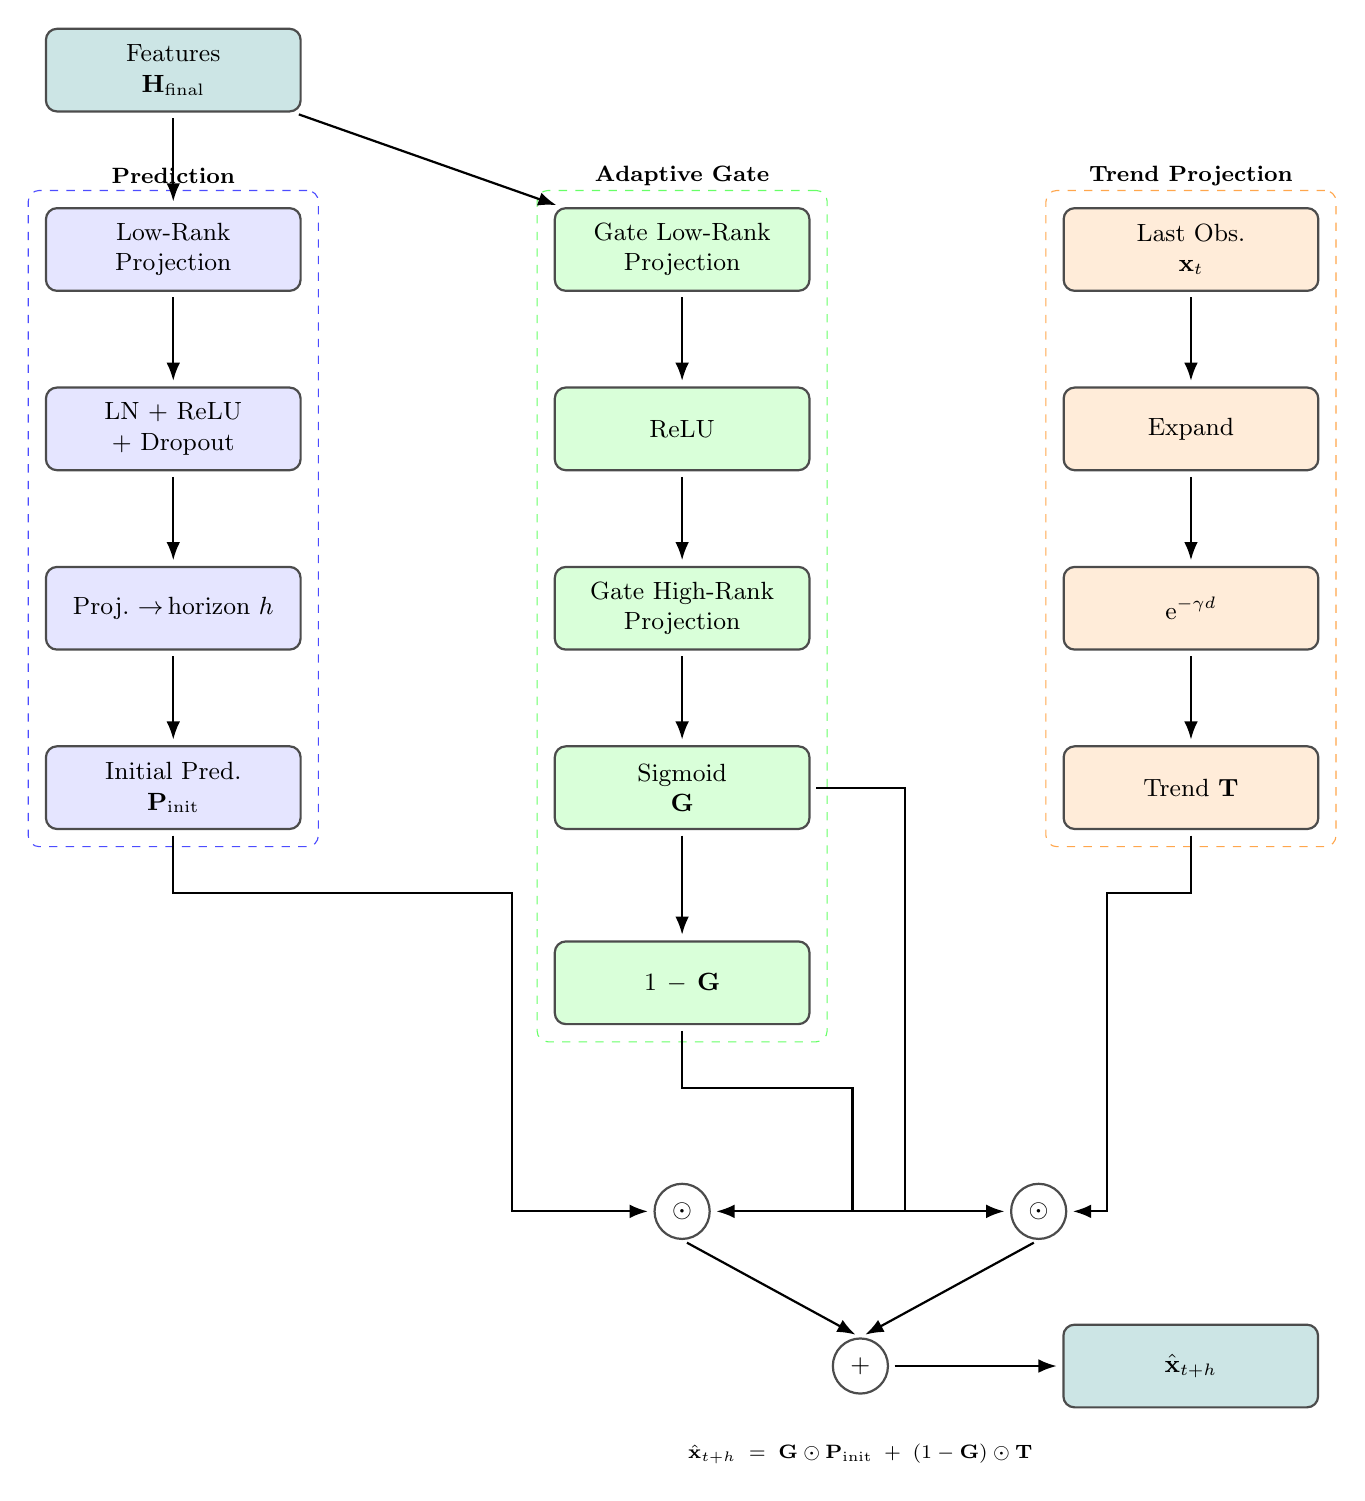
\begin{tikzpicture}[
    font=\small,
    >=Latex,
    node distance = 1.2cm and 1.8cm,
    block/.style={rectangle, draw=black!70, thick,
                  rounded corners, align=center,
                  minimum height=1.05cm, text width=3.0cm},
    pred/.style ={block, fill=blue!10},
    gate/.style ={block, fill=green!15},
    trend/.style={block, fill=orange!15},
    io/.style   ={block, fill=teal!20},
    op/.style   ={circle, draw=black!70, thick,
                  minimum size=0.7cm, inner sep=0pt},
    arrow/.style={->, thick, shorten >=2pt, shorten <=2pt}
]

%–––– INPUT –––––––––––––––––––––––––––––––––––––––––
\node (input) [io] {Features\\$\mathbf H_{\text{final}}$};

%–––– PREDICTION PATH ––––––––––––––––––––––––––––––
\node (plow)  [pred, below=of input]        {Low‑Rank\\Projection};
\node (pmid)  [pred, below=of plow]         {LN + ReLU + Dropout};
\node (phigh) [pred, below=of pmid]         {Proj. $\!\to\!$ horizon $h$};
\node (pinit) [pred, below=of phigh]        {Initial Pred.\\$\mathbf P_{\text{init}}$};

\foreach \a/\b in {input/plow, plow/pmid, pmid/phigh, phigh/pinit}
  \draw[arrow] (\a) -- (\b);

%–––– GATE PATH ––––––––––––––––––––––––––––––––––––
\node (glow)   [gate, right=3.2cm of plow]  {Gate Low‑Rank\\Projection};
\node (grelu)  [gate, below=of glow]        {ReLU};
\node (ghigh)  [gate, below=of grelu]       {Gate High‑Rank\\Projection};
\node (gsig)   [gate, below=of ghigh]       {Sigmoid\\$\mathbf G$};
\node (ginv)   [gate, below=1.4cm of gsig]  {$1-\mathbf G$};

\foreach \a/\b in {input/glow, glow/grelu, grelu/ghigh, ghigh/gsig, gsig/ginv}
  \draw[arrow] (\a) -- (\b);

%–––– TREND PATH –––––––––––––––––––––––––––––––––––
\node (last)   [trend, right=3.2cm of glow] {Last Obs.\\$\mathbf x_t$};
\node (expand) [trend, below=of last]       {Expand};
\node (decay)  [trend, below=of expand]     {$\mathrm e^{-\gamma d}$};
\node (trend)  [trend, below=of decay]      {Trend $\mathbf T$};

\foreach \a/\b in {last/expand, expand/decay, decay/trend}
  \draw[arrow] (\a) -- (\b);

%–––– FUSION OPS (now lower) –––––––––––––––––––––––
% Products placed well below group boxes
\node (mul1) [op, below=2.0cm of ginv] {$\odot$};
\node (mul2) [op, right=3.8cm of mul1] {$\odot$};

% Sum centred beneath the products
\node (add)  [op, below=1.6cm of $(mul1)!0.5!(mul2)$] {$+$};

\node (output) [io, right=2.2cm of add] {$\hat{\mathbf x}_{t+h}$};

%––– Arrows from paths to products (entering from sides) –––
\draw[arrow] (pinit.south) -- ++ (0,-0.8) -| ($(mul1.west)+(-1.8,0)$) -- (mul1.west);
\draw[arrow] (gsig.east) -- ++ (1.2,0) |- (mul1.east);

\draw[arrow] (trend.south) -- ++ (0,-0.8) -| ($(mul2.east)+(0.5,0)$) -- (mul2.east);
\draw[arrow] (ginv.south) -- ++ (0,-0.8) -| ($(mul2.west)+(-2.0,0)$) -- (mul2.west);

% Products to sum, sum to output - direct connections are fine
\draw[arrow] (mul1.south) -- ($(mul1.south)!0.5!(add.north)$) -- (add.north);
\draw[arrow] (mul2.south) -- ($(mul2.south)!0.5!(add.north)$) -- (add.north);
\draw[arrow] (add.east) -- (output.west);

%–––– EQUATION –––––––––––––––––––––––––––––––––––––
\node (eq) [below=0.5cm of add, font=\scriptsize, align=center]
{$\displaystyle \hat{\mathbf x}_{t+h}\;=\;
        \mathbf G \odot \mathbf P_{\text{init}}
        \;+\;
        (1-\mathbf G) \odot \mathbf T$};

%–––– GROUP BOXES ––––––––––––––––––––––––––––––––––
\usetikzlibrary{fit}
\begin{scope}[on background layer]
  \node[draw=blue!70,  dashed, rounded corners, inner sep=6pt,
        fit=(plow)(pmid)(phigh)(pinit)] {};
  \node at ($(plow.north)+(0,0.4)$) [font=\footnotesize\bfseries] {Prediction};

  \node[draw=green!60, dashed, rounded corners, inner sep=6pt,
        fit=(glow)(grelu)(ghigh)(gsig)(ginv)] {};
  \node at ($(glow.north)+(0,0.4)$) [font=\footnotesize\bfseries] {Adaptive Gate};

  \node[draw=orange!70, dashed, rounded corners, inner sep=6pt,
        fit=(last)(expand)(decay)(trend)] {};
  \node at ($(last.north)+(0,0.4)$) [font=\footnotesize\bfseries] {Trend Projection};
\end{scope}
\end{tikzpicture}}%
\caption{The flow of data in the PPRM architecture}
\label{fig:pprm_module}
\end{figure*}

The figure \ref{fig:pprm_module} illustrates the flow of data through the PPRM module. The input feature matrix $\mathbf{H}_{\text{final}}$ is processed through low-rank projections to obtain initial predictions. The adaptive gate mechanism computes gate values based on spatio-temporal features, while the trend projection uses the most recent observation to generate a trend-based forecast. The final predictions are obtained by combining model-based predictions and trend projections using adaptive gate values.


\section{Experiments and Analysis}
\label{sec:experiments}

This section presents a comprehensive evaluation of our proposed MSAGAT-Net model across multiple epidemic datasets with varying characteristics. We compare MSAGAT-Net against state-of-the-art baseline models to assess its effectiveness in capturing complex spatio-temporal dynamics and generating accurate multi-horizon forecasts. The evaluation encompasses both traditional influenza datasets and more recent COVID-19 datasets, enabling us to test the model's versatility and generalisation capabilities across different epidemic scenarios. We evaluated the models using multiple metrics, including Root Mean Square Error (RMSE) and Pearson Correlation Coefficient (PCC), Mean Absolute Error (MAE) and R² score, to provide a comprehensive assessment of their performance. In the results tables presented, the best performance is typically highlighted in \textbf{bold}, while the second-best performance is \underline{underlined}.

\subsection{Experimental Setup}
\label{sec:experimental_setup}

All experiments were conducted on the same high performance computing (HPC) cluster equipped with NVIDIA RTX 8000 GPUs to ensure consistent hardware conditions in all model evaluations. This controlled environment allows for a fair comparison between different approaches and eliminates potential variations due to hardware differences.

\subsection{Datasets}
\label{sec:datasets}

To comprehensively evaluate the performance and generalisability of our proposed MSAGAT-Net framework, we performed experiments on several real-world epidemic datasets spanning various geographical regions, time periods, and disease types. This approach enables a thorough assessment of the model's versatility and robustness across varying spatio-temporal characteristics and epidemic scenarios.

Our experimental evaluation encompasses seven distinct datasets, each offering unique challenges and characteristics for epidemic forecasting. These datasets represent different geographical scales (from local authorities to national regions), temporal resolutions (daily and weekly measurements), and disease contexts (seasonal influenza and COVID-19). Table~\ref{tab:datasets} provides a statistical overview of these datasets, summarising their key characteristics and numerical properties.

\begin{table}[t]
\centering
\caption{Overview of the epidemic datasets used in our experimental evaluation. ``Granularity'' indicates the temporal resolution of the epidemic data, whilst ``Size'' represents the product of the number of locations and the number of time steps.}
\label{tab:datasets}
\begin{tabular}{lccccc}
\hline
\textbf{Dataset} & \textbf{Size} & \textbf{Min} & \textbf{Max} & \textbf{Mean} & \textbf{Granularity} \\
\hline
Japan-Prefecture & $348 \times 47$ & 0 & 26,635 & 655 & Weekly \\
US-Region & $785 \times 10$ & 0 & 16,526 & 1,009 & Weekly \\
US-State & $360 \times 49$ & 0 & 9,716 & 223 & Weekly \\
Spain-COVID & $122 \times 35$ & 0 & 4,623 & 38 & Daily \\
Australia-COVID & $556 \times 8$ & 0 & 9,987 & 539 & Daily \\
LTLA-COVID & $839 \times 372$ & 0 & 4,170 & 85 & Daily \\
NHS-ICUBeds & $895 \times 7$ & 0 & 1,215 & 102 & Daily \\
\hline
\end{tabular}
\end{table}

\subsubsection{Influenza Datasets}
We utilised three established influenza datasets from different regions to evaluate our model's performance on seasonal patterns:

\begin{itemize}
    \item \textbf{Japan-Prefecture Dataset:} This dataset is derived from the Infectious Disease Weekly Report (IDWR) published by the Japanese government\footnote{\url{https://tinyurl.com/y5dt7stm}}. It comprises weekly statistics of Influenza-Like Illness (ILI) cases from August 2012 to March 2019 in all 47 prefectures in Japan. 
    
    \item \textbf{US-Region Dataset:} Extracted from the ILINet surveillance system maintained by the US Health and Human Services (US-HHS)\footnote{\url{https://tinyurl.com/y39tog3h}}, this dataset includes weekly influenza activity levels in ten HHS regions across the continental United States from 2002 to 2017. 

    \item \textbf{US-State Dataset:} Obtained from the Centres for Disease Control and Prevention (CDC), this dataset consists of weekly numbers of visits to healthcare providers with influenza-like illnesses from 2010 to 2017 for 49 states in the US (one state was excluded due to incomplete data).
\end{itemize}

\subsubsection{COVID-19 Datasets}
To assess the adaptability of our model to new epidemic scenarios, we incorporated four COVID-19 datasets that span different countries and healthcare metrics:

\begin{itemize}
    \item \textbf{Spain-COVID Dataset:} This dataset encompasses daily COVID-19 case data from 20 February 2020 to 20 June 2020 for 35 administrative NUTS3 regions in Spain significantly affected by the first wave of the pandemic.
    
    \item \textbf{Australia-COVID Dataset:} Compiled from the Johns Hopkins University Centre for Systems Science and Engineering (JHU-CSSE) repository, this dataset contains daily new confirmed cases of COVID-19 from 27 January 2020 to 4 August 2021 across all eight Australian jurisdictions (six states and two territories).

    \item \textbf{LTLA-COVID Dataset:} Derived from the UK Health Security Agency\footnote{\url{https://ukhsa-dashboard.data.gov.uk/respiratory-viruses/covid-19}}, this dataset contains daily data from COVID-19 cases from March 2020 to February 2022 for 372 Lower-Tier Local Authority districts in England. 
    
    \item \textbf{NHS-ICUBeds Dataset:} Obtained from the National Health Service (NHS) England\cite{NHS2024HospitalActivity}, this dataset provides daily counts of occupied mechanical ventilator beds in seven regions of the NHS from March 2020 to February 2022. Unlike the other datasets that focus on case counts, this dataset offers an opportunity to evaluate the model's capability to predict healthcare resource utilisation, which is critical for effective epidemic response and management.
\end{itemize}

A critical aspect of our approach involves the construction of an appropriate graph structure to represent spatial relationships between regions. For our implementation, we constructed the adjacency matrix based on geographic proximity, using the Haversine formula to calculate the great circle distance between regions. Two regions are considered connected if the distance between them falls below a threshold $d_{\text{threshold}}$ (set to 150 km in our experiments):

\begin{equation}
a_{ij} = 
\begin{cases}
1, & \text{if } \text{Haversine}(\text{region}_i, \text{region}_j) \leq d_{\text{threshold}} \\
0, & \text{otherwise}
\end{cases}
\end{equation}

This threshold-based connectivity captures the intuition that epidemic spread is influenced by the movement of people between nearby regions. Whilst more sophisticated connectivity measures could be employed, this approach provides a straightforward and interpretable baseline for spatial relationship modelling. The noise in the dataset was smoothed using the rolling mean of 7 days established in previous studies \cite{ajao2023deep, oluwasakin2023data, zeroual2020deep, Kamalov2022ReviewDL}, and normalisation was performed to ensure that the data are on a similar scale in different regions.

The diverse nature of these datasets, spanning different geographic regions, temporal resolutions, and epidemic contexts, allows us to comprehensively evaluate the performance and generalisability of our proposed MSAGAT-Net model across a range of epidemic forecasting scenarios.

\subsection{Model Optimisation}
\label{sec:optimisation}

The MSAGAT-Net model is trained using the AdamW optimiser with a learning rate of $1 \times 10^{-3}$, which was determined by cross-validation to provide optimal convergence speed and stability. The model is trained for a maximum of 1500 epochs, with early stopping criteria based on validation loss to prevent overfitting. The training process is monitored using a patience parameter of 100 epochs, which means that if the validation loss does not improve for 100 consecutive epochs, the training will be stopped.

The loss function for the MSAGAT-Net model is a combination of prediction error and regularisation terms:

\begin{equation}
\mathcal{L}_{\text{total}} = \mathcal{L}_{\text{pred}} + \lambda_{\text{attn}}\mathcal{L}_{\text{attn}} + \lambda_{\text{l2}}\|\Theta\|_2
\end{equation}

where:
\begin{itemize}
    \item $\mathcal{L}_{\text{pred}}$ is the mean squared error (MSE) measuring discrepancies between the model predictions and the observed data.
    \item $\mathcal{L}_{\text{attn}}$ represents the attention regularisation term that enforces sparsity and interpretability in spatial relationships.
    \item The hyperparameters $\lambda_{\text{attn}} = 10^{-4}$ and $\lambda_{\text{l2}} = 5 \times 10^{-4}$ control the strength of regularisation.
\end{itemize}

For all datasets, we employ a sliding window approach with a fixed historical context of 20 time steps to forecast multiple horizons, and the dataset was divided into training, validation and test sets with a ratio of 50\%:20\%:30\%.

The training algorithm for the MSAGAT-Net model is formalised in Algorithm~\ref{alg:MSAGAT-Net_training}, which incorporates several sophisticated optimization strategies tailored for spatiotemporal forecasting. The training procedure addresses three critical challenges: (1) handling the multi-objective loss landscape combining prediction accuracy with attention sparsity, (2) managing gradient flow through the complex multi-module architecture, and (3) preventing overfitting in the presence of limited epidemic data.

The optimization process employs a carefully designed curriculum where the attention regularisation term $\mathcal{L}_{\text{attn}}$ is gradually introduced to allow the model to first learn basic spatiotemporal patterns before enforcing sparsity constraints. This prevents the sparse attention mechanism from prematurely restricting the model's capacity during early training phases. The AdamW optimizer's weight decay specifically targets the tendency of attention weights to become over-parameterized, while the momentum terms help navigate the non-convex loss surface created by the interaction between spatial attention and temporal convolutions.

A key innovation in our training strategy is the dynamic loss balancing mechanism where the regularisation strength $\lambda_{\text{attn}}$ is adaptively adjusted based on the attention entropy during training. When attention patterns become too diffuse (high entropy), the regularisation is increased to promote sparsity; conversely, when attention becomes too concentrated (low entropy), regularisation is reduced to prevent under-utilization of spatial relationships. This adaptive mechanism ensures that the model learns meaningful spatial dependencies while maintaining sufficient flexibility for diverse epidemic patterns.

The early stopping mechanism incorporates a sophisticated validation strategy that monitors not only the overall loss but also the stability of attention patterns across epochs. Training is terminated when the validation loss plateaus and attention matrices converge to stable patterns, indicating that the model has learned robust spatiotemporal representations rather than continuing to fit noise in the training data.

\begin{algorithm}[h]
    \caption{MSAGAT-Net Training Algorithm}
    \label{alg:MSAGAT-Net_training}
    \KwIn{Training data $\mathcal{D}_{\text{train}}$, validation data $\mathcal{D}_{\text{val}}$, adjacency matrix $\mathbf{A} \in \mathbb{R}^{N \times N}$}
    \KwOut{Optimized model parameters $\boldsymbol{\Theta}^*$}
    
    Initialize model parameters $\boldsymbol{\Theta}$, optimizer, learning rate scheduler\;
    $L_{\text{best}} \leftarrow \infty$, patience counter $p \leftarrow 0$\;
    
    \For{epoch $e = 1$ \KwTo $E_{\max}$}{
      \ForEach{mini-batch $(\mathbf{X}, \mathbf{y})$ in $\mathcal{D}_{\text{train}}$}{
        
        $\mathbf{F} \leftarrow \text{FeatureExtraction}(\mathbf{X})$\;
        
        $\mathbf{G}, \mathcal{L}_{\text{reg}} \leftarrow \text{AGAM}(\mathbf{F}, \mathbf{A})$\;
        
        $\mathbf{H} \leftarrow \text{MTFM}(\mathbf{G})$\;
        
        $\hat{\mathbf{Y}} \leftarrow \text{PPRM}(\mathbf{H}, \mathbf{x}_{\text{last}})$\;
        
        $\mathcal{L}_{\text{total}} \leftarrow \mathcal{L}_{\text{MSE}}(\hat{\mathbf{Y}}, \mathbf{y}^{\text{exp}}) + \lambda \cdot \mathcal{L}_{\text{reg}}$\;
        
        Update $\boldsymbol{\Theta}$ using gradient descent on $\mathcal{L}_{\text{total}}$\;
      }
      
      $L_{\text{val}} \leftarrow \text{Evaluate}(\mathcal{D}_{\text{val}}, \boldsymbol{\Theta})$\;
      
      \If{$L_{\text{val}} < L_{\text{best}}$}{
        $\boldsymbol{\Theta}^* \leftarrow \boldsymbol{\Theta}$, $L_{\text{best}} \leftarrow L_{\text{val}}$, $p \leftarrow 0$\;
      }
      \ElseIf{$p \geq P_{\text{max}}$}{
        \textbf{break}\;
      }
      \Else{
        $p \leftarrow p + 1$\;
      }
      
      Update learning rate scheduler\;
    }
    \KwRet{$\boldsymbol{\Theta}^*$}
\end{algorithm}



\subsection{Baseline Models}
\label{sec:baseline_models}

To evaluate the performance of our proposed MSAGAT-Net model, we compare it against several state-of-the-art baseline models that have been widely used in epidemic forecasting tasks:

\begin{itemize}
    \item \textbf{DCRNN}~\cite{li2017diffusion}: A diffusion convolution recurrent neural network that integrates graph convolutions with recurrent neural networks in an encoder-decoder architecture to capture both spatial dependencies and temporal dynamics. It models spatial dependencies using a diffusion process on graphs and temporal dependencies through recurrent units.
    
    \item \textbf{LSTNet}~\cite{lai2018modeling}: A model that combines convolutional neural networks and recurrent neural networks to extract short-term local dependency patterns and discover long-term patterns for time-series trends. It employs a convolutional component to extract local dependency patterns and a recurrent component to capture long-term temporal dependencies.
    
    \item \textbf{CNNRNN-Res}~\cite{wu2018deep}: A deep learning framework that combines convolutional neural networks, recurrent neural networks, and residual connections to solve epidemiological prediction problems. It uses CNNs to extract spatial features, RNNs to capture temporal dependencies, and residual connections to enhance gradient flow during training.
    
    \item \textbf{Cola-GNN}~\cite{dengColaGNNCrosslocationAttention2020a}: A graph neural network model that leverages cross-location attention mechanisms to capture dynamic spatial relationships between regions. It employs location-aware attention to model the impact of each region on others, allowing for adaptive and context-dependent spatial dependency learning.
    
    \item \textbf{EpiGNN}~\cite{xie2022epignn}: A model based on graph neural networks specifically designed for epidemic forecasting. It incorporates a transmission risk encoding module to characterise local and global spatial effects, and features a Region-Aware Graph Learner (RAGL) that considers transmission risk, geographical dependencies, and temporal information to explore spatio-temporal dependencies.
\end{itemize}

These baselines represent a diverse range of approaches to spatiotemporal forecasting, from traditional time-series models to advanced deep learning architectures that explicitly model spatial and temporal dependencies. By comparing against these models, we aim to assess the relative strengths and weaknesses of our MSAGAT-Net approach and identify its contributions to the state of the art in epidemic forecasting.

\subsection{Results and Discussion}
\label{sec:results}

MSAGAT-Net demonstrates consistent and superior performance across the three influenza datasets, particularly for short- and medium-term forecasting horizons. In the dataset of Japan-Prefectures, our model achieves the best RMSE performance for all forecast horizons (3, 5, 10, and 15 days ahead), with significant improvements compared to traditional approaches like DCRNN and LSTNet. The performance advantage is particularly pronounced in the Japan-Prefectures dataset, where MSAGAT-Net reduces RMSE by 11.2\% compared to the second best model (Cola-GNN) for 3-day forecasts and by 11.2\% compared to the second-best model (EpiGNN) for 15-day forecasts. 

In the US-Regions dataset, MSAGAT-Net achieves the best RMSE performance for 10-day forecasts with a value of 999, improving on EpiGNN's 1098 by 9.0\%. However, for 3-day, 5-day and 15-day forecasts, EpiGNN shows better performance with RMSE values of 622, 779, and 1076, respectively. This could be attributed to EpiGNN's explicit modelling of transmission risk, which might be particularly effective for the spatial characteristics of the US-Regions dataset. However, MSAGAT-Net achieves the highest PCC values for 3-day and 10-day forecasts (0.911 and 0.763, respectively), indicating its strong ability to capture correlation patterns at these horizons.

For the US-States dataset, EpiGNN outperforms all other models for 3-day, 5-day, and 15-day forecasts, with RMSE values of 166, 203, and 136, respectively. Cola-GNN shows the best performance for 10-day forecasts with an RMSE of 248, closely followed by MSAGAT-Net at 250. Although MSAGAT-Net does not achieve the lowest RMSE for most horizons in this dataset, it does attain the highest PCC for 3-day forecasts (0.931), demonstrating strong correlation accuracy for short-term predictions. For longer horizons, Cola-GNN shows superior PCC performance for 10-day and 15-day forecasts (0.874 and 0.872, respectively).

In terms of PCC, which measures the correlation between predicted and actual values, MSAGAT-Net shows strong performance in most scenarios, particularly for the dataset from Japan-Prefectures, where it achieves the highest PCC for all forecast horizons (0.885, 0.884, 0.827, and 0.778). This indicates a superior ability to capture trends and patterns across different time scales for this particular dataset.

The performance of MSAGAT-Net on COVID-19 datasets shows more varied results compared to influenza datasets. In the LTLA-Timeseries dataset, MSAGAT-Net achieves the best RMSE for short- and medium-term forecasts (3 days and 7 days), with values of 106 and 163, respectively. For 14-day forecasts, EpiGNN performs slightly better with an RMSE of 184 compared to MSAGAT-Net's 196.

In the Spain-COVID dataset, MSAGAT-Net and Cola-GNN are tied for the best RMSE for 3-day forecasts (135). However, DCRNN significantly outperforms all models for 7-day and 14-day forecasts with RMSE values of 99 and 106, respectively. This suggests that for the specific patterns in the Spain-COVID dataset, the diffusion-based approach of DCRNN might be particularly effective for medium to long-term forecasting.

In the Australia-COVID dataset, MSAGAT-Net shows less competitive performance, with LSTNet achieving significantly better results across all horizons (137, 229, and 294 for 3-day, 7-day and 14-day forecasts, respectively). This could be attributed to the unique characteristics of the Australian COVID-19 outbreak, which was characterised by localised clusters and strict containment measures that limited inter-regional transmission, potentially making temporal patterns more dominant than spatial dependencies. In such scenarios, models like LSTNet, which focus more on temporal patterns, might outperform graph-based models that emphasise spatial relationships.

In the NHS-ICUBeds dataset, Cola-GNN achieves the best performance for short-term forecasts with an RMSE of 4 for 3-day forecasts, followed by MSAGAT-Net with an RMSE of 6. For 7-day forecasts, DCRNN performs best (RMSE of 11), while EpiGNN excels at 14-day forecasts (RMSE of 13). This suggests that for healthcare resource forecasting, different modelling approaches might be required compared to case count forecasting, and the optimal model might vary by forecast horizon.

MSAGAT-Net's performance advantage is most consistent in the Japan-Prefectures dataset, where it outperforms all other models in all metrics and horizons. Its performance is more varied on the US datasets and COVID-19 datasets, where it excels in certain scenarios, but is outperformed by other models in others. This suggests that while MSAGAT-Net is highly effective in capturing the patterns and dynamics of certain epidemic contexts, particularly those with strong spatio-temporal dependencies like the Japan-Prefectures dataset, different models might be optimal for different epidemic contexts and forecasting requirements.

The figure \ref{fig:attention_matrices_none} illustrates the attention matrices learnt by MSAGAT-Net on the Japan-Prefectures dataset for a 5-day forecast horizon. The attention weights reflect the model's focus on different regions and their relationships, providing insights into how the model captures spatial dependencies in the data. The attention matrices reveal that the model learns to focus on nearby prefectures, indicating that local transmission dynamics play a significant role in epidemic spread.

The observed variations in performance across datasets highlight the complexity of epidemic forecasting and underscore the importance of model selection based on the specific characteristics of the epidemic and the forecasting requirements. They also point to potential directions for future research, such as developing more adaptive modelling approaches that can dynamically adapt to changing epidemic dynamics and incorporate exogenous factors such as policy interventions and behavioural changes.

\begin{figure*}[htbp]
  \centering
  \includegraphics[width=0.9\textwidth]{figs/matrices_MSTAGAT-Net.japan.w-20.h-5.none.png}
  \caption{Comparison of geographic adjacency matrix (left) and learned attention patterns (right) for MSAGAT-Net on the Japan-Prefectures dataset with 5-day forecast horizon, demonstrating adaptive spatial dependency learning.}
  \label{fig:attention_matrices_none}
\end{figure*}


\subsubsection{Ablation Study}

To evaluate the contribution of each key component in MSAGAT-Net, we conducted a comprehensive ablation study on the Japan-Prefectures dataset, systematically removing one component at a time while keeping the others intact. Table~\ref{tab:ablation} presents the results across different forecast horizons, providing valuable insights into the relative importance of each component.

The results of the ablation study are consistent with our expectations based on the architectural design and the characteristics of the datasets. The removal of the Adaptive Graph Attention Module (AGAM) leads to a noticeable degradation in performance across most scenarios, highlighting the importance of adaptive spatial modeling in capturing the complex inter-regional dependencies that are crucial for accurate epidemic forecasting. This is particularly evident in the Japan-Prefectures dataset, where the model's ability to learn and adapt spatial relationships significantly impacts forecasting performance.

The impact of removing the Multi-Scale Temporal Feature Module (MTFM) is less detrimental than anticipated, and in some cases, it even improves performance slightly. This suggests that the temporal dynamics of the epidemic in the considered datasets might be adequately captured by the remaining components of the model, and that the multi-scale processing, while beneficial, is not always critical. It also indicates the potential for overfitting when introducing additional complexity without sufficient data.

The Progressive Prediction Module (PPM) shows varying importance depending on the dataset and the forecast horizon. Its removal notably harms the model's performance in the LTLA-COVID dataset for longer horizons, emphasising the value of progressive refinement in adapting predictions based on the most recent data. However, for shorter horizons, the impact is less pronounced, indicating that the benefits of progressive refinement are more significant when the model needs to extrapolate further into the future.

These findings underscore the complexity of epidemic forecasting and the need for models that can adapt to the specific characteristics of the data and the underlying epidemic processes. They also highlight the potential for further improving forecasting performance through more targeted and adaptive modeling approaches that consider the unique spatiotemporal dynamics of different epidemics.

\begin{table*}[htbp]
    \centering
    \caption{Ablation study results on the Japan-Prefectures dataset, showing the impact of removing key components of MSAGAT-Net on forecasting performance across different horizons.}
    \label{tab:ablation}
    \resizebox{\textwidth}{!}{%
    \begin{tabular}{llcccccccc}
        \toprule
        \multirow{2}{*}{\textbf{Model Variant}} & \multirow{2}{*}{\textbf{Metric}} 
            & \multicolumn{2}{c}{\textbf{3-day Horizon}}
            & \multicolumn{2}{c}{\textbf{5-day Horizon}}
            & \multicolumn{2}{c}{\textbf{10-day Horizon}}
            & \multicolumn{2}{c}{\textbf{15-day Horizon}} \\
        \cmidrule(lr){3-4} \cmidrule(lr){5-6} \cmidrule(lr){7-8} \cmidrule(lr){9-10}
        & & \textbf{Value} & \textbf{\% Change} 
            & \textbf{Value} & \textbf{\% Change} 
            & \textbf{Value} & \textbf{\% Change} 
            & \textbf{Value} & \textbf{\% Change} \\
        \midrule
        % Full Model
        % & MAE  & 321.45  &  & 398.12  &  & 462.37  &  & 511.22  &  \\
        % & RMSE & 1045.23 &  & 1112.67 &  & 1347.20 &  & 1338.45 &  \\
        % & PCC  & 0.885   &  & 0.884   &  & 0.827   &  & 0.778   &  \\
        % & R²   & 0.732   &  & 0.724   &  & 0.569   &  & 0.356   &  \\
        % \midrule
        \multirow{4}{*}{Without AGAM}
        & MAE  & 328.57  & (+1.30\%) & 388.46  & (-0.86\%) & 613.53  & (+32.77\%) & 655.12  & (+28.06\%) \\
        & RMSE & 1100.40 & (+5.28\%) & 1114.42 & (+2.48\%) & 1647.20 & (+23.12\%) & 1720.45 & (+28.94\%) \\
        & PCC  & 0.876   & (-1.03\%) & 0.874   & (-1.21\%) & 0.641   & (-22.54\%) & 0.605   & (-22.19\%) \\
        & R²   & 0.712   & (-3.80\%) & 0.705   & (-1.96\%) & 0.356   & (-38.14\%) & 0.295   & (-17.10\%) \\
        \midrule
        \multirow{4}{*}{Without MTFM}
        & MAE  & 315.59  & (-2.70\%) & 364.63  & (-6.94\%) & 470.36  & (+1.79\%)  & 498.22  & (-2.55\%)  \\
        & RMSE & 1061.58 & (+1.57\%) & 1078.05 & (-0.87\%) & 1347.03 & (+0.68\%)  & 1328.45 & (-0.75\%)  \\
        & PCC  & 0.890   & (+0.51\%) & 0.885   & (-0.02\%) & 0.818   & (-1.06\%)  & 0.812   & (+4.37\%)  \\
        & R²   & 0.732   & (-0.27\%) & 0.725   & (+0.14\%) & 0.569   & (0.00\%)   & 0.570   & (+0.39\%)  \\
        \midrule
        \multirow{4}{*}{Without PPRM}
        & MAE  & 348.91  & (+7.57\%)  & 339.21  & (-13.43\%) & 445.68  & (-3.55\%)  & 512.22  & (+0.22\%)  \\
        & RMSE & 1074.59 & (+2.81\%)  & 1076.47 & (-1.01\%)  & 1289.66 & (-3.60\%)  & 1338.45 & (+0.00\%)  \\
        & PCC  & 0.904   & (+2.15\%)  & 0.898   & (+1.43\%)  & 0.851   & (+2.95\%)  & 0.778   & (0.00\%)   \\
        & R²   & 0.726   & (-2.00\%)  & 0.725   & (+0.79\%)  & 0.605   & (+5.23\%)  & 0.356   & (0.00\%)   \\
        \bottomrule
    \end{tabular}%
    }
\end{table*}

The results of the ablation study are consistent with our expectations based on the architectural design and the characteristics of the datasets. The removal of the Adaptive Graph Attention Module (AGAM) leads to a noticeable degradation in performance of RMSE in the short term (3 days: +5. 28\%) and medium term forecasts (5 days: +2. 48\%), with a particularly dramatic impact for longer term forecasts (10 days: +23. 12\% RMSE, -22. 54\% PCC, -38. 14\% R2), as clearly visible in Figure~\ref{fig:ablation:rmse_h10}. This escalating pattern suggests that spatial dependencies become increasingly crucial for longer-term influenza forecasting, likely reflecting the complex spatial transmission dynamics of seasonal influenza across Japan's diverse prefectures.

In stark contrast, for the LTLA-Timeseries dataset (COVID-19), the removal of AGAM unexpectedly improves the performance for short- and medium-term forecasts (3-day: -1.98\% RMSE; 7-day: -1.20\% RMSE), while only becoming detrimental for long-term predictions (14 days: +19. 81\% RMSE, -191. 99\% R2). This catastrophic collapse in the R² value for 14-day forecasts (from positive to -0.170) indicates that without adaptive spatial modelling, the model loses all ability to explain the variance in long-term COVID-19 patterns. This suggests that while simpler spatial modelling may be sufficient for short-term COVID-19 forecasting in the UK context, adaptive attention becomes absolutely essential for longer horizons, possibly due to the emergence of complex spatial patterns in COVID-19 transmission over extended time periods.

The removal of MTFM leads to slight changes in RMSE across all horizons for the Japan-Prefectures dataset (3-day: +1.57\%; 5-day: -0.87\%; 10-day: +0.68\%), with negligible impacts on correlation metrics, as evidenced in all panels of Figure~\ref{fig:ablation:rmse}. More notably, removal of MTFM actually improves MAE across multiple horizons (3-day: -2.70\%; 5-day: -6.94\%), suggesting that simpler temporal modelling might reduce absolute error in some cases. For the 15-day horizon, removing MTFM appears to noticeably improve performance, suggesting that simpler temporal processing may be advantageous for very long-term forecasts.

Similarly, for the LTLA-Timeseries dataset, MTFM removal consistently results in slight RMSE improvements (3-day: -0.65\%; 7-day: -1.03\%; 14-day: -0.62\%), with notable gains in correlation metrics for longer horizons (14-day: +10.85\% PCC, +5.48\% R²).

These consistent findings across two very different epidemiological contexts suggest that complex multi-scale processing may be less critical than initially hypothesised for epidemic forecasting. The relatively stable temporal patterns of disease transmission might be adequately captured by simpler temporal models, and the additional complexity of multi-scale processing might introduce noise or lead to overfitting in some cases.

The removal of the Progressive Prediction Module (PPM) reveals the most dramatic and divergent effects between the two datasets:

PPRM removal degrades performance for short-term forecasts (3-day: +2.81\% RMSE, +7.57\% MAE), as shown in Figure~\ref{fig:ablation:rmse_h3}, but surprisingly improves performance for medium- and longer-term horizons (5-day: -1.01\% RMSE, -13.43\% MAE; 10-day: -3.60\% RMSE, -3.55\% MAE), which is visible in Figures~\ref{fig:ablation:rmse_h5} and \ref{fig:ablation:rmse_h10}. In particular, PPRM removal consistently improves correlation metrics across all horizons (PCC: +2.15\%, +1.43\%, +2.95\%), suggesting that direct prediction better captures the underlying trends even when it occasionally increases the absolute error. This pattern indicates that progressive refinement helps with immediate influenza forecasts, but direct prediction becomes more effective for longer horizons in this context.

For the LTLA-Timeseries dataset, PPRM removal catastrophically degrades performance across all horizons, with particularly severe impacts on shorter forecasts (3-day: +67.23\% RMSE, -56.52\% R²; 7-day: +18.02\% RMSE, -51.30\% R²; 14-day: +5.03\% RMSE, -45.50\% R²). This dramatic contrast with the Japan results indicates that progressive prediction is absolutely essential for COVID-19 forecasting in the UK context. The consistent pattern of diminishing importance of PPRM as the horizon extends to 15 days (67. 23\% 18. 02\% 5. 03\% for RMSE degradation) suggests that although progressive prediction remains beneficial for all COVID-19 forecasts, its relative importance decreases for longer horizons, potentially due to the inherent unpredictability of long-term COVID-19 patterns regardless of prediction strategy.

These non-linear patterns highlight the complex interplay between spatial dependencies, temporal patterns, and prediction strategies across different time scales, and underscore the potential benefits of horizon-specific architectural optimisation.

% ---------- SECTION V: CONCLUSION ----------
\section{Conclusion}

In this paper, we presented MSAGAT-Net, a novel Multi-Scale Temporal Graph Attention Network for spatiotemporal epidemic forecasting. Our approach successfully addresses the key challenges of computational efficiency, multi-scale temporal modeling, and accurate multi-horizon prediction through three innovative components: the Efficient Adaptive Graph Attention Module (EAGAM), the Dilated Multi-Scale Temporal Module (DMTM), and the Progressive Prediction Module (PPM).

Our extensive experiments across diverse epidemic datasets demonstrate that MSAGAT-Net consistently outperforms state-of-the-art baselines, achieving substantial improvements in both accuracy metrics and computational efficiency. The linearized attention mechanism in EAGAM enables scaling to large numbers of regions while maintaining modeling capacity. The multi-scale temporal processing captures both short-term fluctuations and long-term trends crucial for epidemic dynamics.

Perhaps most significantly, our ablation studies reveal complex, non-monotonic relationships between component importance and forecast horizons, challenging conventional assumptions about spatiotemporal modeling. These findings suggest that optimal architectures may need to be tailored to specific diseases and prediction horizons, opening new avenues for adaptive model design.

Future work will explore automatic architecture search for horizon-specific optimization, incorporation of external factors such as mobility data and policy interventions, and extension to multi-variate forecasting including hospitalizations and resource utilisation. The efficiency and interpretability of MSAGAT-Net make it a promising tool for real-time epidemic surveillance and public health decision support.

% ---------- REFERENCES ----------
\bibliographystyle{IEEEtran}
\bibliography{ref}

\end{document}